% !TEX encoding = UTF-8 Unicode
\documentclass[fontsize=11pt, paper=A4, pagesize=auto, oneside]{book}
\usepackage[utf8]{inputenc}
\usepackage[spanish,mexico]{babel}
\usepackage{subfiles}
\usepackage[nottoc,notlot,notlof]{tocbibind}
\usepackage{graphicx}
\usepackage{capt-of}
\usepackage{amsmath}
\usepackage{tabu}
\usepackage{titling}
\usepackage[hidelinks]{hyperref}
\usepackage[toc,page]{appendix}
\usepackage{color}
\usepackage{enumitem}
\usepackage[toc]{glossaries}
\usepackage{caption}

\makeatletter
\newcommand*{\textlabel}[2]{%
  \edef\@currentlabel{#1}% Set target label
  \phantomsection% Correct hyper reference link
  #1\label{#2}% Print and store label
}
\makeatother

\begin{document}
	\renewcommand{\bibname}{Referencias}
	\setcounter{secnumdepth}{5}
	
	\begin{titlepage}
    \begin{minipage}{0.15\textwidth}
    	
\includegraphics[width=0.8\textwidth]{Portada/img/ipn.jpg}
    \end{minipage}
    \begin{minipage}{0.65\textwidth}
        \begin{center}
            \large \bf Instituto Politécnico Nacional \newline
            \large \bf Escuela Superior de Cómputo \newline
        \end{center}
    \end{minipage}
    \begin{minipage}{0.20\textwidth}
        
\includegraphics[width=.9\textwidth]{Portada/img/escom.jpg}
    \end{minipage}
    
    \vspace{1cm}
    
    \centering
    \Large{Trabajo Terminal No. 2016 - B030\\Sistema móvil de detección de alcohol en conductores, con bloqueo automotriz} \par
    
    \vspace{1cm}
    
    \large{Cazares Curiel Jorge Armando\\Diaz Rodarte Juan Gerardo\\Porras Velázquez Jorge Armando} \par
    
    \vspace{1cm}
    
	\small{Dirigido por}\par
	\normalsize{Rubén Ortega González\\Carranza Castillo Oscar}
    
\end{titlepage}
	
	\tableofcontents
	% Índice de figuras y tablas
	\listoffigures
	\listoftables
	
	% Capitulo 1: Planteamiento del Problema
	\chapter{Planteamiento del problema}
En este capítulo se planteara el problema que se busca resolver a traves de nuestro trabajo terminal, así como los objetivos, justificación y resultados esperados.
	\subfile{Capitulo1/introduccion}
	\subfile{Capitulo1/objetivo}
	\subfile{Capitulo1/justificacion}
	\subfile{Capitulo1/resultados}
	
	% Capitulo 2: Estado del Arte
	\chapter{Estado del Arte}
En este capítulo se dara una breve introducción a la alcoholemia, la tecnología y los dispositivos para el análisis del alcohol en la sangre y una comparación con proyectos similares.Estado anímico alterado (Mayor bienestar o infelicidad)
Amistoso, timidez y argumentativo
Concentración y juicio deteriorado
Desinhibición sexual

	\subfile{Capitulo2/alcoholemia}
	%\subfile{Capitulo2/comparacion}
	
	% Capitulo3
	\chapter{ANÁLISIS}
En este capítulo se realizará el análisis de requerimientos funcionales y no funcionales para la aplicación móvil mediante diagrama de casos de uso, de secuencia, etc. con el propósito de generar un esquema a seguir en la etapa de implementación.
	\subfile{Capitulo3/herramientas}
	\subfile{Capitulo3/requerimientos}
	\subsection{Requerimientos Funcionales} 
  
  \begin{center}
   \begin{tabular}{|p{5.5cm}|p{7cm}|}
     \hline
     \multicolumn{2}{|c|}{De la aplicación móvil} \\ \hline
     \\ RF01-AM  \\ ENLAZAR DISPOSITIVO ELECTRÓNICO & Descripción: Se vinculará la aplicación móvil con el dispositivo de detección de alcohol \\ \\ \hline
     \\ RF02-AM \\ REGISTRAR CONTACTOS & Descripción: se registran contactos dentro de la aplicación paa comunicar el estado del conductor, los cuales recibirán un mensaje de texti \\ \\ \hline
   \end{tabular}
 \end{center}  


  
    \begin{center}
   \begin{tabular}[b]{| p{5.5cm} | p{7cm} |}
     \hline
     \multicolumn{2}{|c|}{Del dispositivo de detección de alcohol} \\ \hline
     \\ RF01-DDA \\ ENLAZAR CON LA APLICACIÓN MÓVIL & Descripción: Se vinculará el dispositivo con la aplicación móvil \\ \\ \hline
     \\ RF02-DDA \\ RECIBE MUESTRA & Descripción: Se recibirá las muestras a través de un contacto físico con el dispositivo \\ \\ \hline
     \\ RF03-DDA \\ ANALIZA MUESTRA & Descripción: El dispositivo analizará una señal para detectar los niveles de etanol y retornará un valor que será validado en la aplicación \\ \\ \hline
     \\ RF04-DDA \\ ENVÍAR RESULTADO & Descripción: Se envía el resultado a la aplicación para verificar si está en condiciones para poder manejar \\ \\ \hline
     \\ RF05-DDA \\ INMOVILIZADOR & Descripción: Una vez que se detecta que no se encuentra el conductor en condiciones para manejar, se realizará
  un corte de gasolina para que el carro no pueda arrancar \\ \\ \hline
   \end{tabular}
 \end{center}

	\subsection{Requerimientos No Funcionales} 
  
\textbf{Dispositivo de detección de alcohol}
\begin{center}
\begin{table}[!htb]
\centering
\begin{tabular}{|p{4cm}|p{4cm}|p{5cm}|}
    \hline
    \centering {\bfseries }  & \centering {\bfseries Nombre} & {\bfseries Descripción} \\ \hline
    \centering RNF06-RDDA & \centering Características del dispositivo & Los elementos que formarán parte del dispositivo deberán tener las siguientes características: \\ \hline
    \centering RNF07-RDDA & \centering Comunicación con la aplicación & Para poder establecer la comunicación, es necesario tener instalada la aplicación \\ \hline
    \centering RNF08-PDDA & \centering Tamaño del dispositivo & El tamaño debe ser pequeño, de tal manera que se pueda adaptar a alguna parte del automóvil \\ \hline
\end{tabular}
\caption{Requerimientos no funcionales - Restricciones}
\label{tabla:pobconlimsincolo}
\end{table}
\end{center}

\begin{center}
\begin{table}[!htb]
\centering
\begin{tabular}{|p{4cm}|p{4cm}|p{5cm}|}
    \hline
    \centering {\bfseries }  & \centering {\bfseries Nombre} & {\bfseries Descripción} \\ \hline
    \centering RNF08-PDDA & \centering Tamaño del dispositivo & El tamaño debe ser pequeño, de tal manera que se pueda adaptar a alguna parte del automóvil \\ \hline
\end{tabular}
\caption{Requerimientos no funcionales - Propiedades}
\label{tabla:pobconlimsincolo}
\end{table}
\end{center}

\textbf{Aplicación móvil}
\begin{center}
\begin{table}[!htb]
\centering
\begin{tabular}{|p{4cm}|p{4cm}|p{5cm}|}
    \hline
    \centering {\bfseries }  & \centering {\bfseries Nombre} & {\bfseries Descripción} \\ \hline
    \centering RNF01-RAM & \centering Lenguaje de programación & Se utilizará el lenguaje java y xml junto con el SDK oficial para desarrollar la aplicación para dispositivos con sistema Android \\ \hline
    \centering RNF02-RAM & \centering Sistema operativo & Para ejecutar la aplicación será necesario contar Android desde la versión 4.0\\ \hline
\end{tabular}
\caption{Requerimientos no funcionales - Restricciones}
\label{tabla:pobconlimsincolo}
\end{table}
\end{center}
    

\begin{center}
\begin{table}[!htb]
\centering
\begin{tabular}{|p{4cm}|p{4cm}|p{5cm}|}
    \hline
    \centering {\bfseries }  & \centering {\bfseries Nombre} & {\bfseries Descripción} \\ \hline
    \centering RNF01-PAM & \centering Interfaz Gráfica & Se realizará una interfaz gráfica para la interacción con el usuario \\ \hline 
    \centering RNF02-PAM &  \centering Comunicación & La comunicación dispositivo-aplicación se realizará mediante \\
    \hline
\end{tabular}
\caption{Requerimientos no funcionales - Propiedades}
\label{tabla:pobconlimsincolo}
\end{table}
\end{center}

	\subsection{Análisis de Riesgos}


	\subfile{Capitulo3/diagramas_casos_de_uso}
	\section{Casos de Uso}
Los casos de uso que se presentan a continuación pretenden capturar el comportamiento del sistema, dividiendo la funcionalidad en transacciones que realizarán los diferentes actores (personas, otros sitemas informáticos y procesos).
\subsection{Caso de uso 1: Iniciar sesión} \label{cu1}
\subsubsection{Resumen}
Este caso de uso le permite al actor ingresar al sistema proporcionando su nombre de usuario y contraseña para poder realizar las funciones correspondientes a su perfil.
\subsubsection{Descripción}
\begingroup
\setlength{\LTleft}{-10cm plus -1fill}
\setlength{\LTright}{\LTleft}
\begin{center}  
  \captionof{table}{Caso de uso 1: Iniciar sesión } \label{tab:cu1_tab}
  \begin{longtable}{| p{3.5cm} | p{11.5cm} |}
      	\hline
      		\textbf{Versión} &  0.1 \\
        \hline 
       		\textbf{Autor} & Juan Gerardo Diaz Rodarte\\
        \hline
          \textbf{Estatus} & Edición \\
        \hline  
          \textbf{Fecha de último estatus} &  3 de abril de 2017 \\
        \hline
      \multicolumn{2}{|c|}{\large{Atributos}} \\
        \hline
          \textbf{Actor}  & Administrador, Usuario y Sub-Usuario. \\
        \hline	
          \textbf{Propósito} & Permite a los diferentes actores ingresar al sistema. \\
        \hline
          \textbf{Disparador} & El actor abre la aplicación y presiona el botón de Iniciar sesión. \\
        \hline	
          \textbf{Entradas} & 
            \begin{itemize}
              \item \textbf{Correo electrónico}: Se escribe con el teclado.
              \item \textbf{Contraseña}: Se escribe con el teclado.
            \end{itemize} \\
        \hline	
          \textbf{Salidas} & 
            \begin{itemize}
              \item \textbf{Interna}: Se redirecciona a la vista de inicio IU.
            \end{itemize} \\
        \hline	
          \textbf{Precondiciones}& 
            \begin{itemize}
              \item \textbf{Interna:} El actor debe estar registrado en el sistema.
            \end{itemize} \\
        \hline	
          \textbf{Postcondiciones} & 
            \begin{itemize}
              \item \textbf{Interna:} Al actor se le otorgan permisos para realizar actividades de acuerdo a su perfil y es redireccionado. 
		\begin{itemize}
			\item El Administrador sera redireccionado al IU Index.
			\item Para el Usuario y Sub-Usuario se redireccionara al IU Index.
		\end{itemize}
            \end{itemize} \\
       \hline
         \textbf{Reglas de negocio} & 
         	\begin{itemize}
         	  \item \textbf{\ref{rnl_01}}
         	  \item \textbf{\ref{rnl_02}}
         	  \item \textbf{\ref{rnrv_01}}
         	  \item \textbf{\ref{rnrv_02}}
         	  \item \textbf{\ref{rnrv_03}}
	 \end{itemize} \\
       \hline
         \textbf{Mensajes} & 
         	\begin{itemize}
         	  \item \textbf{\ref{msja_01}}
         	  \item \textbf{\ref{msje_01}}
         	  \item \textbf{\ref{msje_02}}
	 \end{itemize} \\
       \hline
         \textbf{Tipo} & Primario \\
    \hline	    
  \end{longtable}
\end{center}
\endgroup

\subsubsection{Trayectorias del caso de uso}
\textbf{Trayectoria principal}
\begin{enumerate}
  \item {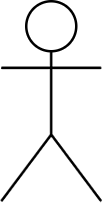
\includegraphics[scale=.1]{Capitulo3/img/actor.png} Ingresa el actor a la aplicación móvil, en el caso del administrador ingresa al portal web mediante una dirección eletrónica.}
  \item {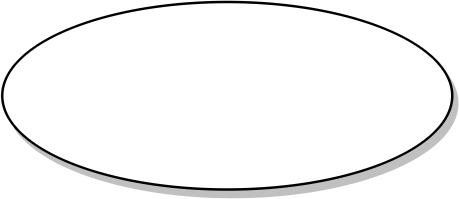
\includegraphics[scale=.05]{Capitulo3/img/proceso.png} Se muestar la vista IU Index para el administrador y IU Inicio para los demás actores.}
  \item {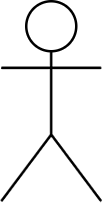
\includegraphics[scale=.1]{Capitulo3/img/actor.png} Presiona el botón de Iniciar sesión.}
  \item {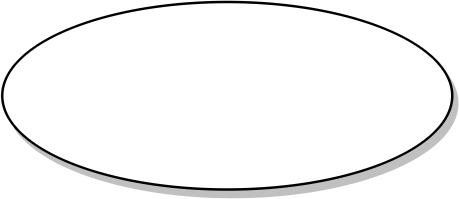
\includegraphics[scale=.05]{Capitulo3/img/proceso.png} Se redirecciona a la vista IU Iniciar sesión.}
  \item {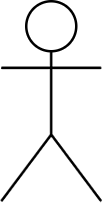
\includegraphics[scale=.1]{Capitulo3/img/actor.png} Ingresa el la dirección de correo electrónico y contraseña en los campos correspondientes.}
  \item {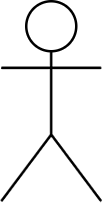
\includegraphics[scale=.1]{Capitulo3/img/actor.png} Presiona el botón para solicitar ingresar al sistema.}
  \item {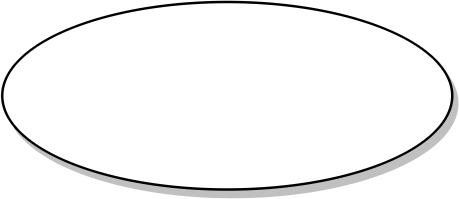
\includegraphics[scale=.05]{Capitulo3/img/proceso.png} Verifica que el usuario haya ingresado la información requerida como establecido en la \textbf{\ref{rnl_01}}. \hyperref[cu1_ta_a]{[Trayectoria alternativa A]}}
  \item {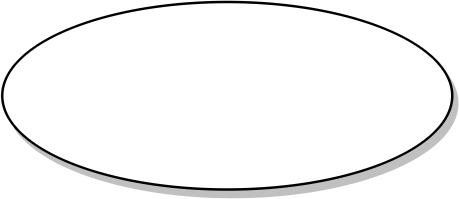
\includegraphics[scale=.05]{Capitulo3/img/proceso.png} Verifica que la dirección de correo eletrónico y la contraseña sean válidos de acuerdo a las reglas de negocio correspondientes. \hyperref[cu1_ta_b]{[Trayectoria alternativa B]} \hyperref[cu1_ta_c]{[Trayectoria alternativa C]}}
  \item {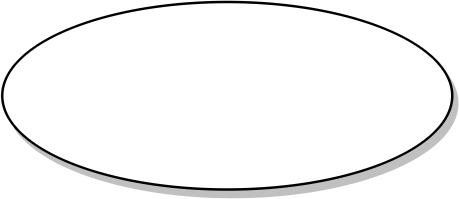
\includegraphics[scale=.05]{Capitulo3/img/proceso.png} Verifica que la dirección de correo eletrónico y la contraseña coincidan con aquellos datos registrados en el sistema. \hyperref[cu1_ta_d]{[Trayectoria alternativa D]} \hyperref[cu1_ta_e]{[Trayectoria alternativa E]}}
  \item {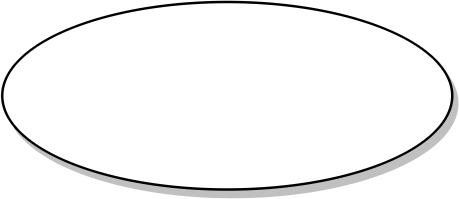
\includegraphics[scale=.05]{Capitulo3/img/proceso.png} Se muestra la vista de inicio correspondiente al actor.}
  \item {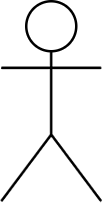
\includegraphics[scale=.1]{Capitulo3/img/actor.png} Hacer uso del sistema.}\\
  \textit{Fin de caso de uso} \\	
\end{enumerate}

\textbf{Trayectoria alternativa A} \phantomsection\label{cu1_ta_a} \\
\textbf{Condición:} El actor no proporcionó la información requerida, rompiendo la regla de negocio \textbf{\ref{rnl_01}}.\\
 \begin{enumerate}[label=A\arabic*]
    \item {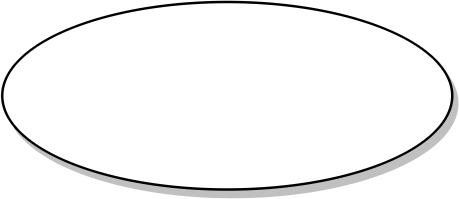
\includegraphics[scale=.05]{Capitulo3/img/proceso.png} Muestra el mensaje \textbf{\ref{msja_01}}, indicando que el actor ha dejado campos en blanco.}
    \item {Continua en el paso 5 de la trayectoria principal.} \\
    \textit{Fin de trayectoria} \\
\end{enumerate}

\textbf{Trayectoria alternativa B} \phantomsection\label{cu1_ta_b}\\
\textbf{Condición:} El actor no ingreso una dirección de correo electrónico que cumpla con la regla de negocio \textbf{\ref{rnrv_02}}.\\
 \begin{enumerate}[label=B\arabic*]
    \item {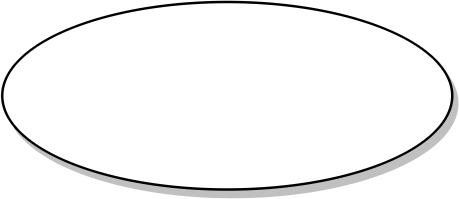
\includegraphics[scale=.05]{Capitulo3/img/proceso.png} Muestra el mensaje \textbf{\ref{msje_02}}, indicando que la dirección de correo electrónico no es válida.}
    \item {Continua en el paso 5 de la trayectoria principal.} \\
    \textit{Fin de trayectoria} \\
\end{enumerate}

\textbf{Trayectoria alternativa C} \phantomsection\label{cu1_ta_c}\\
\textbf{Condición:} El actor ingreso una contraseña incorrecta que no cumple con la regla de negocio \textbf{\ref{rnrv_03}}.\\
 \begin{enumerate}[label=C\arabic*]
    \item {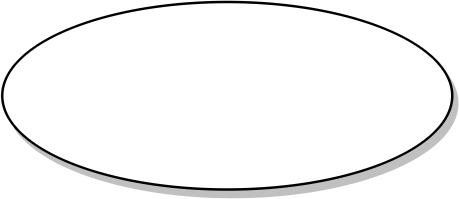
\includegraphics[scale=.05]{Capitulo3/img/proceso.png} Muestra el mensaje \textbf{\ref{msje_01}}, indicando que el actor ha ingresado datos incorrectos.}
    \item {Continua en el paso 5 de la trayectoria principal.} \\
    \textit{Fin de trayectoria} \\
\end{enumerate}

\textbf{Trayectoria alternativa D} \phantomsection\label{cu1_ta_d}\\
\textbf{Condición:} No se encontró alguna cuenta relacionada con la dirección de correo electrónico ingresada de acuerdo a la regla de negocio \textbf{\ref{rnrv_01}}.\\
 \begin{enumerate}[label=D\arabic*]
    \item {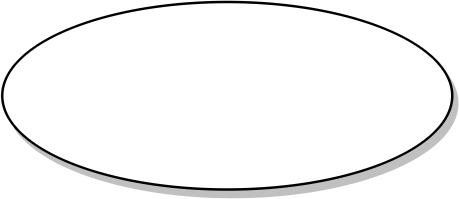
\includegraphics[scale=.05]{Capitulo3/img/proceso.png} Muestra el mensaje \textbf{\ref{msje_01}}, indicando que el actor ha ingresado datos incorrectos en alguno de los campos.}
    \item {Continua en el paso 5 de la trayectoria principal.} \\
    \textit{Fin de trayectoria} \\
\end{enumerate}

\textbf{Trayectoria alternativa E} \phantomsection\label{cu1_ta_e}\\
\textbf{Condición:} La contraseña ingresada no corresponde a la cuenta de la dirección de correo electrónico ingresada de acuerdo a la regla de negocio \textbf{\ref{rnrv_01}}.\\
 \begin{enumerate}[label=E\arabic*]
    \item {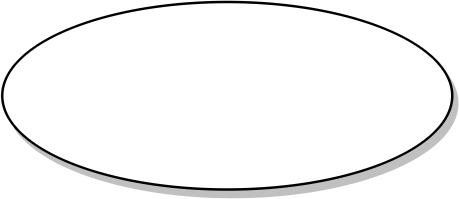
\includegraphics[scale=.05]{Capitulo3/img/proceso.png} Muestra el mensaje \textbf{\ref{msje_01}}, indicando que el actor ha ingresado datos incorrectos en alguno de los campos.}
    \item {Continua en el paso 5 de la trayectoria principal.} \\
    \textit{Fin de trayectoria} \\
\end{enumerate}

\textbf{Trayectoria alternativa F} \phantomsection\label{cu1_ta_f}\\
\textbf{Condición:} El actor selecciono la opción de \textit{¿Has olvidado tu contraseña?}.\\
 \begin{enumerate}[label=F\arabic*]
    \item {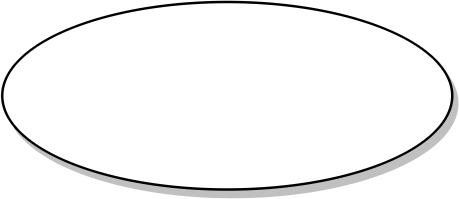
\includegraphics[scale=.05]{Capitulo3/img/proceso.png} Se ejecuta el \hyperref[cu1_1]{CU 1.1 Recuperar contraseña}} \\
    \textit{Fin de trayectoria} \\
\end{enumerate}

\textbf{Trayectoria alternativa G} \phantomsection\label{cu1_ta_g}\\
\textbf{Condición:} El actor selecciono la opción de \textit{¿Eres nuevo aquí?}.\\
 \begin{enumerate}[label=G\arabic*]
    \item {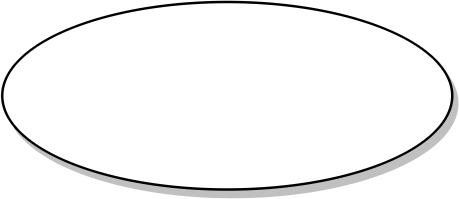
\includegraphics[scale=.05]{Capitulo3/img/proceso.png} Se ejecuta el \hyperref[cu2]{CU 2 Registrarse}} \\
    \textit{Fin de trayectoria} \\
\end{enumerate}

\subsubsection{Puntos de extensión}
\noindent \textbf{Causa de la extensión:} El actor, de tipo de Usuario o Sub-Usuario, selecciono \textit{¿Has olvidado tu contraseña?} \\
\textbf{Región de la trayectoria:} \hyperref[cu1_ta_f]{Trayectoria alternativa F} \\
\textbf{Extiende a:} \hyperref[cu1_1]{CU 1.1 Recuperar contraseña} \\ \par

\noindent \textbf{Causa de la extensión:} El actor, de tipo de Usuario o Sub-Usuario, selecciono \textit{¿Eres nuevo aquí?} \\
\textbf{Región de la trayectoria:} \hyperref[cu1_ta_G]{Trayectoria alternativa G} \\
\textbf{Extiende a:} \hyperref[cu2]{CU 2 Registrarse}

\newpage
\subsection{Caso de uso 1.1: Recuperar contraseña} \label{cu1_1}
\subsubsection{Resumen}
Este caso de uso permite al actor ingresar una dirección de correo electrónico con la cual podrá recuperar su contraseña.
\subsubsection{Descripción}
\begingroup
\setlength{\LTleft}{-10cm plus -1fill}
\setlength{\LTright}{\LTleft}
\begin{center}
    \addtocounter{table}{-1}
    \captionof{table}{Caso de uso 1.1: Recuperar contraseña} \label{tab:cu1_1_tab}
	\begin{longtable}{| p{3.5cm} | p{11.5cm} |}
      	\hline
      		\textbf{Versión} &  0.1 \\
        \hline 
       		\textbf{Autor} & Juan Gerardo Diaz Rodarte\\
        \hline
          \textbf{Estatus} & Edición \\
        \hline  
          \textbf{Fecha de último estatus} & 29 de marzo de 2017 \\
        \hline
      \multicolumn{2}{|c|}{\large{Atributos}} \\
        \hline
          \textbf{Actor} & Usuario y Sub-Usuario. \\
        \hline	
          \textbf{Propósito} & Permite a los actores registrados ingresar al sistema. \\
        \hline
          \textbf{Disparador} & Al presionar el botón BTN en la vista IU Registrate o IU Iniciar sesión. \\
        \hline	
          \textbf{Entradas} & 
            \begin{itemize}
              \item Correo electrónico: Se escribe con el teclado.
            \end{itemize} \\
        \hline	
          \textbf{Salidas} & 
            \begin{itemize}
              \item Interna: Se mostrará el mensaje MSG que indica que el correo ha sido enviado.
            \end{itemize} \\
        \hline	
          \textbf{Precondiciones}& 
            \begin{itemize}
              \item \textbf{Interna:} El actor debe estar registrado en el sistema.
            \end{itemize} \\
        \hline	
          \textbf{Postcondiciones} & 
            \begin{itemize}
              \item \textbf{Interna:} Un correo electrónico será enviado al actor con el cual podrá recuperar su contraseña.
            \end{itemize} \\
       \hline    
          \textbf{Reglas de negocio} & 
          \begin{itemize}
         	  \item {\hyperref[rnr_04]{RNR 04: Campos obligatorios}}
         	  \item {\hyperref[rnr_01]{RNE 01: Cuenta válida}}
         	  \item {\hyperref[rnr_02]{RNE 02: Dirección de correo electrónico válido}}
	 \end{itemize} \\
       \hline
          \textbf{Mensajes} & 
         	\begin{itemize}
         	  \item {\hyperref[msje_01]{MSJE 01: Datos inválidos}}
         	  \item {\hyperref[msje_02]{MSJE 02: Correo electrónico inválido}}
         	  \item {\hyperref[msja_01]{MSJA 01: Campos en blanco}}
	 \end{itemize} \\
       \hline
          \textbf{Tipo} & Secundario \\
       \hline	    
  \end{longtable}
\end{center}
\endgroup

\subsubsection{Trayectorias del caso de uso}
\textbf{Trayectoria principal}
\begin{enumerate}
  \item {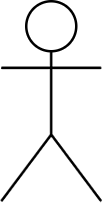
\includegraphics[scale=.1]{Capitulo3/img/actor.png} Ingresa el actor a la aplicación móvil, en el caso del administrador ingresa al portal web mediante una dirección eletrónica.}
  \item {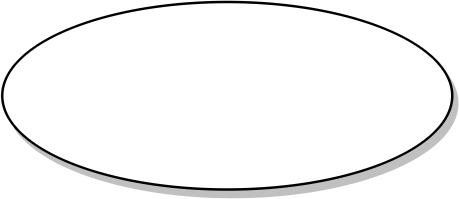
\includegraphics[scale=.05]{Capitulo3/img/proceso.png} Se muestar la vista IU Index para el administrador y IU Inicio para los demás actores.}
  \item {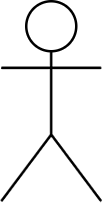
\includegraphics[scale=.1]{Capitulo3/img/actor.png} Presiona el botón de Iniciar sesión.}
  \item {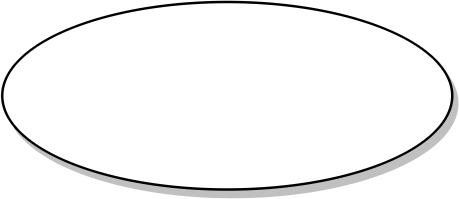
\includegraphics[scale=.05]{Capitulo3/img/proceso.png} Se muestar la vista IU Inicio.}
  \item {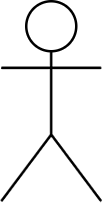
\includegraphics[scale=.1]{Capitulo3/img/actor.png} Selecciona el usuario la opción de \textit{¿Has olvidado tu contraseña}}
  \item {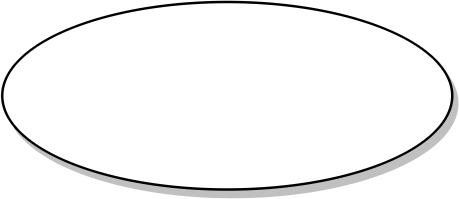
\includegraphics[scale=.05]{Capitulo3/img/proceso.png} El actor ingresa una dirección de correo electrónico.}
  \item {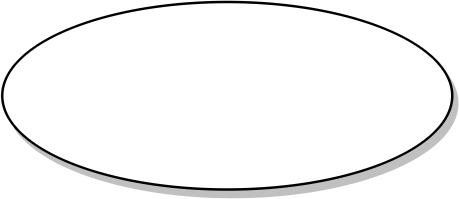
\includegraphics[scale=.05]{Capitulo3/img/proceso.png} Verifica que el usuario haya ingresado la información requerida. \hyperref[cu1_1_ta_a]{[Trayectoria alternativa A]}}
  \item {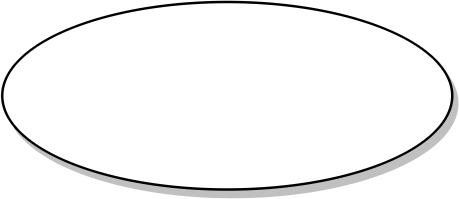
\includegraphics[scale=.05]{Capitulo3/img/proceso.png} Verifica que la dirección de correo electrónico sea una válida. \hyperref[cu1_1_ta_b]{[Trayectoria alternativa B]}}
  \item {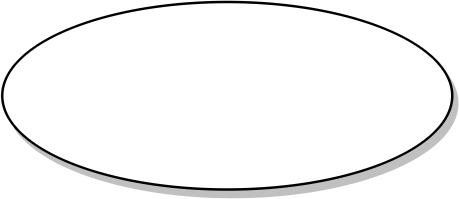
\includegraphics[scale=.05]{Capitulo3/img/proceso.png} Verifica que la dirección de correo eletrónico coincida con alguna cuenta registrada en el sistema. \hyperref[cu1_1_ta_c]{[Trayectoria alternativa C]}}
  \item {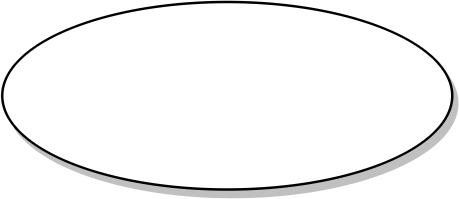
\includegraphics[scale=.05]{Capitulo3/img/proceso.png} Muestra el mensaje MSG, indicando que el correo electrónico ha sido enviado exitosamente.}
  \item {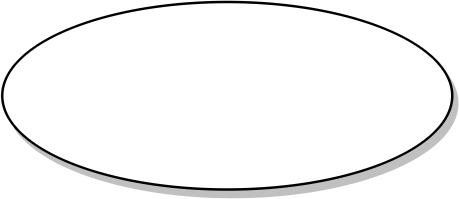
\includegraphics[scale=.1]{Capitulo3/img/proceso.png} Se redirecciona a la vista de inicio de sesión IU Iniciar sesión.} \\
  \textit{Fin de caso de uso} \\	
\end{enumerate}

\textbf{Trayectoria alternativa A} \phantomsection\label{cu1_1_ta_a} \\
\textbf{Condición:} El actor no proporcionó la información requerida, rompiendo la regla de negocio \hyperref[rnr_04]{RNR 04}.\\
 \begin{enumerate}[label=A\arabic*]
    \item {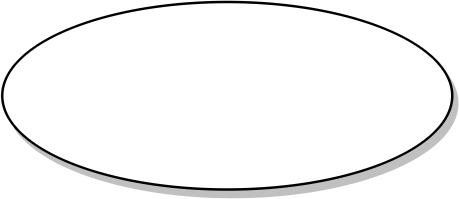
\includegraphics[scale=.05]{Capitulo3/img/proceso.png} Muestra el mensaje \hyperref[msja_01]{MSJA 01}, indicando que el actor ha dejado campos en blanco.}
    \item {Continua en el paso 6  de la trayectoria principal.} \\
    \textit{Fin de trayectoria} \\
\end{enumerate}

\textbf{Trayectoria alternativa B} \phantomsection\label{cu1_1_ta_b}\\
\textbf{Condición:} El actor no ingreso una dirección de correo electrónico que cumpla con la regla de negocio \hyperref[rne_02]{RNE 02}.\\
 \begin{enumerate}[label=B\arabic*]
    \item {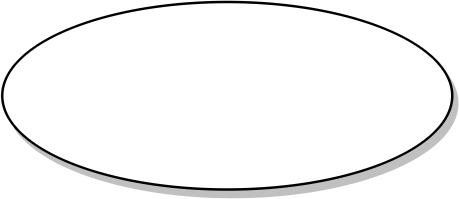
\includegraphics[scale=.05]{Capitulo3/img/proceso.png} Muestra el mensaje \hyperref[msje_02]{MSJE 02}, indicando que la dirección de correo electrónico no es válida.}
    \item {Continua en el paso 6 de la trayectoria principal.} \\
    \textit{Fin de trayectoria} \\
\end{enumerate}

\textbf{Trayectoria alternativa C} \phantomsection\label{cu1_1_ta_c}\\
\textbf{Condición:} No se encontró alguna cuenta relacionada con la dirección de correo electrónico ingresada de acuerdo a la regla de negocio \hyperref[rne_01]{RNE 01}.\\
 \begin{enumerate}[label=C\arabic*]
    \item {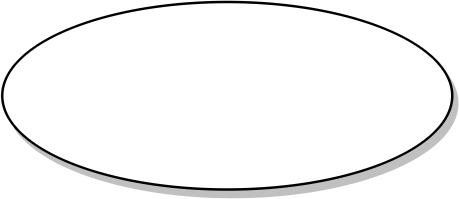
\includegraphics[scale=.05]{Capitulo3/img/proceso.png} Muestra el mensaje \hyperref[msje_01]{MSJE 01}, indicando que el actor ha ingresado datos incorrectos en alguno de los campos.}
    \item {Continua en el paso 6 de la trayectoria principal.} \\
    \textit{Fin de trayectoria} \\
\end{enumerate}

\textbf{Trayectoria alternativa D} \phantomsection\label{cu1_1_ta_d}\\
\textbf{Condición:} El actor selecciono la opción de \textit{¿Eres nuevo aquí?}.\\
 \begin{enumerate}[label=D\arabic*]
    \item {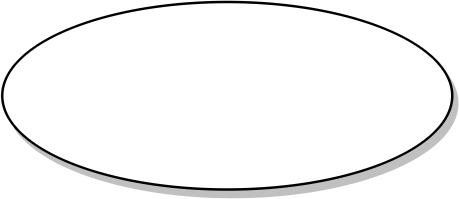
\includegraphics[scale=.05]{Capitulo3/img/proceso.png} Se ejecuta el \hyperref[cu2]{CU 2 Registrarse}} \\
    \textit{Fin de trayectoria} \\
\end{enumerate}

\textbf{Trayectoria alternativa E} \phantomsection\label{cu1_1_ta_e}\\
\textbf{Condición:} El actor selecciono la opción de \textit{¿Ya tienes una cuenta?}.\\
 \begin{enumerate}[label=E\arabic*]
    \item {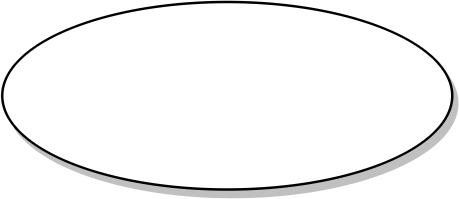
\includegraphics[scale=.05]{Capitulo3/img/proceso.png} Se ejecuta el\hyperref[cu1]{ CU 1 Iniciar sesión.}} \\
    \textit{Fin de trayectoria} \\
\end{enumerate}

\subsubsection{Puntos de extensión}
\noindent \textbf{Causa de la extensión:} El actor, de tipo de Usuario o Sub-Usuario, selecciono \textit{¿Eres nuevo aquí?} \\
\textbf{Región de la trayectoria:} \hyperref[cu1_1_ta_d]{Trayectoria alternativa D} \\
\textbf{Extiende a:} \hyperref[cu1_1]{CU 2 Registrarse} \\ \par

\noindent \textbf{Causa de la extensión:} El actor, de tipo de Usuario o Sub-Usuario, selecciono \textit{¿Ya tienes una cuenta?} \\
\textbf{Región de la trayectoria:} \hyperref[cu1_1_ta_e]{Trayectoria alternativa e} \\
\textbf{Extiende a:} \hyperref[cu1]{CU 1 Iniciar sesión}

\newpage
\subsection{Caso de uso 2: Registrarse} \label{cu2}
\subsubsection{Resumen}
Este caso de uso le permite al usuario registrarse en el sistema proporcionando los datos solicitados.
\subsubsection{Descripción}
\begingroup
\setlength{\LTleft}{-10cm plus -1fill}
\setlength{\LTright}{\LTleft}
\begin{center}
  \addtocounter{table}{-1}
  \captionof{table}{Caso de uso 2: Registrarse} \label{tab:cu2_tab}
  \begin{longtable}{| p{3.5cm} | p{11.5cm} |}
      	\hline
      		\textbf{Versión} &  0.1 \\
        \hline 
       		\textbf{Autor} & Juan Gerardo Diaz Rodarte\\
        \hline
          \textbf{Estatus} & Edición \\
        \hline  
          \textbf{Fecha de último estatus} &  3 de abril de 2017 \\
        \hline
      \multicolumn{2}{|c|}{\large{Atributos}} \\
        \hline
          \textbf{Actor} & Usuario. \\
        \hline	
          \textbf{Disparador} & El actor abre la aplicación y presiona el botón de ¿Eres nuevo aquí?. \\
        \hline
          \textbf{Disparador} & El actor se registro exitosamente y es redirecionado. \\
        \hline
          \textbf{Entradas} & 
            \begin{itemize}
              \item \textbf{Correo electrónico}: Se escribe con el teclado.
              \item \textbf{Contraseña}: Se escribe con el teclado.
              \item \textbf{Confirmar contraseña}: Se escribe con el teclado.
              \item \textbf{Nombre(s)}: Se escribe con el teclado.
              \item \textbf{Apellido Paterno}: Se escribe con el teclado.
              \item \textbf{Apellido Materno}: Se escribe con el teclado.
              \item \textbf{Telefóno}: Se ingresa el código de país con un selector y el número con el teclado.
              \item \textbf{Fecha de nacimiento}: Se selecciona el año, mes y día con un selector.
            \end{itemize} \\
        \hline	
          \textbf{Salidas} &  
          \begin{itemize}
              \item \textbf{Interna}: Se mostrará el mensaje \textbf{\ref{msjn_04}} que indica que el registro fue exitoso.
            \end{itemize} \\
        \hline	
          \textbf{Precondiciones}& 
            \begin{itemize}
              \item \textbf{Interna:} El usuario debe de llenar todos los campos requeridos según la RNO.
            \end{itemize} \\
        \hline	
          \textbf{Postcondiciones} & 
            \begin{itemize}
              \item \textbf{Interna:} Al usuario se le generará una cuenta que necesita ser confirmada.
            \end{itemize} \\
        \hline    
           \textbf{Reglas de negocio} & 
             \begin{itemize}
               \item \textbf{\ref{rnl_01}}
               \item \textbf{\ref{rnl_02}}
               \item \textbf{\ref{rnl_03}}
               \item \textbf{\ref{rnl_04}}
               \item \textbf{\ref{rnl_05}}
               \item \textbf{\ref{rnl_06}}
               \item \textbf{\ref{rnrv_02}}
               \item \textbf{\ref{rnrv_03}}
               \item \textbf{\ref{rnrv_04}}
               \item \textbf{\ref{rnrv_05}}
               \item \textbf{\ref{rnrv_06}}
               \item \textbf{\ref{rnrv_07}}
               \item \textbf{\ref{rnrv_08}}
             \end{itemize} \\
        \hline
           \textbf{Mensajes} & 
              \begin{itemize}
                 \item \textbf{\ref{msja_01}}
                 \item \textbf{\ref{msje_02}}
                 \item \textbf{\ref{msje_03}}
                 \item \textbf{\ref{msje_04}}
                 \item \textbf{\ref{msje_05}}
                 \item \textbf{\ref{msje_06}}
                 \item \textbf{\ref{msje_07}}
                 \item \textbf{\ref{msje_08}}
                 \item \textbf{\ref{msjn_04}}
              \end{itemize}\\
        \hline
           \textbf{Tipo} & Primario \\
        \hline	    
  \end{longtable}
\end{center}
\endgroup

\subsubsection{Trayectorias del caso de uso}
\textbf{Trayectoria principal}
\begin{enumerate}
  \item {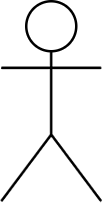
\includegraphics[scale=.1]{Capitulo3/img/actor.png} Ingresa el actor a la aplicación móvil, en el caso del administrador ingresa al portal web mediante una dirección eletrónica.}
  \item {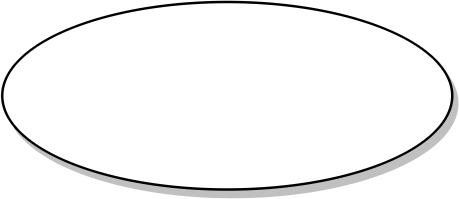
\includegraphics[scale=.05]{Capitulo3/img/proceso.png} Se muestar la vista IU Hogar. \hyperref[cu2_ta_a]{[Trayectoria alternativa A]}}
  \item {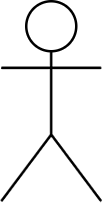
\includegraphics[scale=.1]{Capitulo3/img/actor.png} Selecciona el usuario la opción de \textit{¿Eres nuevo aquí?}}
  \item {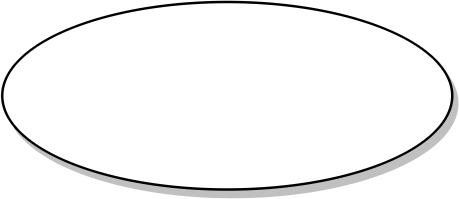
\includegraphics[scale=.05]{Capitulo3/img/proceso.png} Se muestar la vista IU Registro.}
  \item {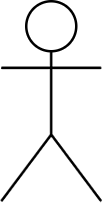
\includegraphics[scale=.1]{Capitulo3/img/actor.png} El actor ingresa los campos requeridos.}
  \item {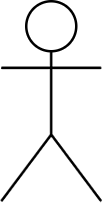
\includegraphics[scale=.1]{Capitulo3/img/actor.png} Presiona el botón para solicitar su registro al sistema.}
  \item {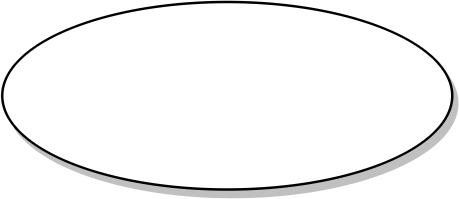
\includegraphics[scale=.05]{Capitulo3/img/proceso.png} Verifica que el usuario haya ingresado la información requerida como establecido en la \hyperref[rnr_04]{RNR 04}. \hyperref[cu2_ta_b]{[Trayectoria alternativa B]}}
  \item {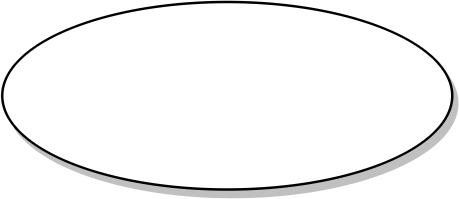
\includegraphics[scale=.05]{Capitulo3/img/proceso.png} Verifica que la dirección de correo electrónico cumpla con la \textbf{\ref{rnrv_02}}. \hyperref[cu2_ta_c]{[Trayectoria alternativa C]}}
  \item {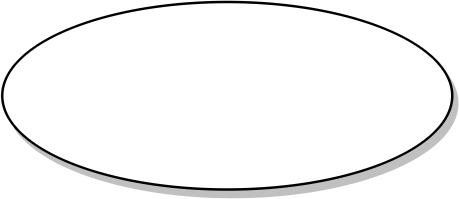
\includegraphics[scale=.05]{Capitulo3/img/proceso.png} Verifica que la contraseña cumpla con la \textbf{\ref{rnrv_03}}. \hyperref[cu2_ta_d]{[Trayectoria alternativa D]}}
  \item {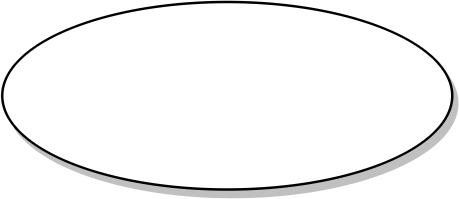
\includegraphics[scale=.05]{Capitulo3/img/proceso.png} Verifica que la contraseña de confirmación coincida con la contrasea ingresada. \hyperref[cu2_ta_e]{[Trayectoria alternativa E]}}
  \item {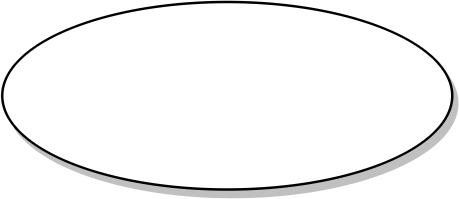
\includegraphics[scale=.05]{Capitulo3/img/proceso.png} Verifica que el nombre cumpla con la \textbf{\ref{rnrv_04}}. \hyperref[cu2_ta_f]{[Trayectoria alternativa F]} \hyperref[cu2_ta_g]{[Trayectoria alternativa G]}}
  \item {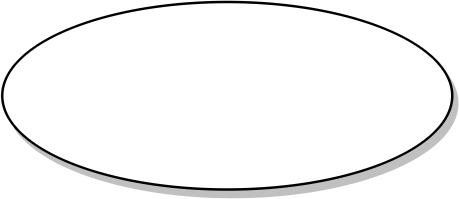
\includegraphics[scale=.05]{Capitulo3/img/proceso.png} Verifica que el apellido paterno cumpla con la \textbf{\ref{rnrv_04}}. \hyperref[cu2_ta_h]{[Trayectoria alternativa H]} \hyperref[cu2_ta_i]{[Trayectoria alternativa I]}}
  \item {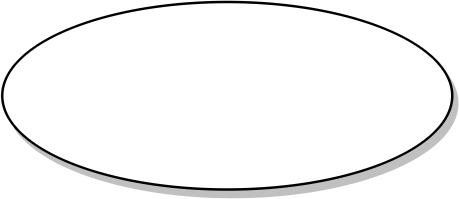
\includegraphics[scale=.05]{Capitulo3/img/proceso.png} Verifica que el apellido materno cumpla con la \textbf{\ref{rnrv_04}}. \hyperref[cu2_ta_h]{[Trayectoria alternativa H]} \hyperref[cu2_ta_i]{[Trayectoria alternativa I]}}
  \item {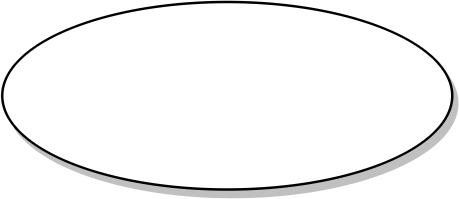
\includegraphics[scale=.05]{Capitulo3/img/proceso.png} Verifica que el teléfono sea válido. \hyperref[cu2_ta_j]{[Trayectoria alternativa J]}}
  \item {\includegraphics[scale=.05]{Capitulo3/img/proceso.png} Verifica que la fecha de nacimiento cumpla con la \textbf{\ref{=rnrv_08}}. \hyperref[cu2_ta_k]{[Trayectoria alternativa K]}}
  \item {\includegraphics[scale=.05]{Capitulo3/img/proceso.png} Se muestra el mensaje \textbf{\ref{msjn_04}} que indica el registro exitoso al sistema.}
  \item {\includegraphics[scale=.1]{Capitulo3/img/proceso.png} Se redirecciona a la vista IU Confirma tu teléfono.}\\
  \textit{Fin de caso de uso} \\	
\end{enumerate}

\textbf{Trayectoria alternativa A} \phantomsection\label{cu2_ta_a} \\
\textbf{Condición:} El actor presiona la opción de \textit{Iniciar sesión}.\\
 \begin{enumerate}[label=A\arabic*]
  \item {\includegraphics[scale=.1]{Capitulo3/img/actor.png} Presiona el botón de Iniciar sesión.}
  \item {\includegraphics[scale=.05]{Capitulo3/img/proceso.png} Se muestar la vista IU Iniciar sesión.}
    \item {Continua en el paso 3 de la trayectoria principal.} \\
    \textit{Fin de trayectoria} \\
\end{enumerate}

\textbf{Trayectoria alternativa B} \phantomsection\label{cu2_ta_b} \\
\textbf{Condición:} El actor no proporcionó la información requerida, rompiendo la regla de negocio \textbf{\ref{rnl_01}}.\\
 \begin{enumerate}[label=B\arabic*]
    \item {\includegraphics[scale=.05]{Capitulo3/img/proceso.png} Muestra el mensaje \textbf{\ref{msja_01}}, indicando que el actor ha dejado campos en blanco.}
    \item {Continua en el paso 5  de la trayectoria principal.} \\
    \textit{Fin de trayectoria} \\
\end{enumerate}

\textbf{Trayectoria alternativa C} \phantomsection\label{cu2_ta_c}\\
\textbf{Condición:} El actor no ingreso una dirección de correo electrónico que cumpla con la regla de negocio \textbf{\ref{rnrv_02}}.\\
 \begin{enumerate}[label=C\arabic*]
    \item {\includegraphics[scale=.05]{Capitulo3/img/proceso.png} Muestra el mensaje \textbf{\ref{msje_02}}, indicando que la dirección de correo electrónico no es válida.}
    \item {Continua en el paso 5 de la trayectoria principal.} \\
    \textit{Fin de trayectoria} \\
\end{enumerate}

\textbf{Trayectoria alternativa D} \phantomsection\label{cu2_ta_d}\\
\textbf{Condición:} El actor ingreso una contraseña incorrecta que no cumple con la regla de negocio \textbf{\ref{rnrv_03}}.\\
 \begin{enumerate}[label=D\arabic*]
    \item {\includegraphics[scale=.05]{Capitulo3/img/proceso.png} Muestra el mensaje \textbf{\ref{msje_01}}, indicando que el actor ha ingresado datos incorrectos.}
    \item {Continua en el paso 5 de la trayectoria principal.} \\
    \textit{Fin de trayectoria} \\
\end{enumerate}

\textbf{Trayectoria alternativa E} \phantomsection\label{cu2_ta_e}\\
\textbf{Condición:} El acto no ingreso la misma contraseña en los campo \textit{Contraseña} y \textit{Confirmar contraseña} coincidan.\\
 \begin{enumerate}[label=E\arabic*]
    \item {\includegraphics[scale=.05]{Capitulo3/img/proceso.png} Muestra el mensaje \textbf{\ref{msje_04}}, indicando que las contraseñas no coinciden.}
    \item {Continua en el paso 5 de la trayectoria principal.} \\
    \textit{Fin de trayectoria} \\
\end{enumerate}

\textbf{Trayectoria alternativa F} \phantomsection\label{cu2_ta_f}\\
\textbf{Condición:} El actor no ingreso un nombre que cumpla con la longitud establecida en la \textbf{\ref{rnl_03}}.\\
 \begin{enumerate}[label=F\arabic*]
    \item {\includegraphics[scale=.05]{Capitulo3/img/proceso.png} Muestra el mensaje \textbf{\ref{msje_05}}, indicando que el nombre sobrepasa la longitud máxima.}
    \item {Continua en el paso 5 de la trayectoria principal.} \\
    \textit{Fin de trayectoria} \\
\end{enumerate}

\textbf{Trayectoria alternativa G} \phantomsection\label{cu2_ta_g}\\
\textbf{Condición:} El actor ingreso un nombre que contiene símbolos o carácteres de tipo númericos.\\
 \begin{enumerate}[label=G\arabic*]
    \item {\includegraphics[scale=.05]{Capitulo3/img/proceso.png} Muestra el mensaje \textbf{\ref{msje_06}}, indicando que el nombre contiene carácteres de tipo númerico o símbolos.}
    \item {Continua en el paso 5 de la trayectoria principal.} \\
    \textit{Fin de trayectoria} \\
\end{enumerate}

\textbf{Trayectoria alternativa H} \phantomsection\label{cu2_ta_h}\\
\textbf{Condición:} El actor no ingreso un apellido que cumpla con la longitud establecida en la \textbf{\ref{rnl_04}} .\\
 \begin{enumerate}[label=H\arabic*]
    \item {\includegraphics[scale=.05]{Capitulo3/img/proceso.png} Muestra el mensaje \textbf{\ref{msje_05}}, indicando que alguno de los apellidos sobrepasa la longitud máxima.}
    \item {Continua en el paso 5 de la trayectoria principal.} \\
    \textit{Fin de trayectoria} \\
\end{enumerate}

\textbf{Trayectoria alternativa I} \phantomsection\label{cu2_ta_i}\\
\textbf{Condición:} El actor ingreso un apellido que contiene símbolos o carácteres de tipo númericos.\\
 \begin{enumerate}[label=I\arabic*]
    \item {\includegraphics[scale=.05]{Capitulo3/img/proceso.png} Muestra el mensaje \hyperref[msje_06]{MSJE 06}, indicando que el apellido contiene carácteres de tipo númerico o símbolos.}
    \item {Continua en el paso 5 de la trayectoria principal.} \\
    \textit{Fin de trayectoria} \\
\end{enumerate}

\textbf{Trayectoria alternativa J} \phantomsection\label{cu2_ta_j}\\
\textbf{Condición:} El actor ingreso teléfono que no coincide con la longitud establecida en la \hyperref[rnrv_05]{RNRV 05} y \hyperref[rnrv_06]{RNRV 06} ó \hyperref[rnrv_07]{RNRV 07} .\\
 \begin{enumerate}[label=J\arabic*]
    \item {\includegraphics[scale=.05]{Capitulo3/img/proceso.png} Muestra el mensaje \textbf{\ref{msje_07}}, indicando que la longitud del número celular es inválida.}
    \item {Continua en el paso 5 de la trayectoria principal.} \\
    \textit{Fin de trayectoria} \\
\end{enumerate}

\textbf{Trayectoria alternativa K} \phantomsection\label{cu2_ta_k}\\
\textbf{Condición:} El actor ingreso una fecha de nacimiento que no cumple con la \textbf{\ref{rnrv_08}}.\\
 \begin{enumerate}[label=K\arabic*]
    \item {\includegraphics[scale=.05]{Capitulo3/img/proceso.png} Muestra el mensaje \textbf{\ref{msje_07}}, indicando que la longitud del número celular es inválida.}
    \item {Continua en el paso 5 de la trayectoria principal.} \\
    \textit{Fin de trayectoria} \\
\end{enumerate}

\textbf{Trayectoria alternativa L} \phantomsection\label{cu2_ta_l}\\
\textbf{Condición:} El actor selecciono la opción de \textit{¿Has olvidado tu contraseña?}.\\
 \begin{enumerate}[label=L\arabic*]
    \item {\includegraphics[scale=.05]{Capitulo3/img/proceso.png} Se ejecuta el \nameref{cu1_1}} \\
    \textit{Fin de trayectoria} \\
\end{enumerate}

\textbf{Trayectoria alternativa M} \phantomsection\label{cu2_ta_m}\\
\textbf{Condición:} El actor selecciono la opción de \textit{¿Ya tienes una cuenta?}.\\
 \begin{enumerate}[label=M\arabic*]
    \item {\includegraphics[scale=.05]{Capitulo3/img/proceso.png} Se ejecuta el \nameref{cu1}}\\
    \textit{Fin de trayectoria} \\
\end{enumerate}

\subsubsection{Puntos de extensión}
\noindent \textbf{Causa de la extensión:} El actor, de tipo de Usuario o Sub-Usuario, selecciono \textit{¿Has olvidado tu contraseña?} \\
\textbf{Región de la trayectoria:} \hyperref[cu2_ta_l]{Trayectoria alternativa L} \\
\textbf{Extiende a:} \nameref{cu1_1} \\ \par

\noindent \textbf{Causa de la extensión:} El actor, de tipo de Usuario o Sub-Usuario, selecciono \textit{¿Ya tienes una cuenta?} \\
\textbf{Región de la trayectoria:} \hyperref[cu2_ta_m]{Trayectoria alternativa M} \\
\textbf{Extiende a:} \nameref{cu1}

\newpage
\subsection{Caso de uso 2.1: Confirmar teléfono celular} \label{cu2_1}
\subsubsection{Resumen}
Este caso de uso le permite al usuario confirmar su teléfono celular ingresando el código que fue enviado al número que proporciono al registrarse.
\subsubsection{Descripción}
\begingroup
\setlength{\LTleft}{-10cm plus -1fill}
\setlength{\LTright}{\LTleft}
\begin{center}
  \addtocounter{table}{-1}
    \captionof{table}{Caso de uso 2.1: Confirmar cuenta} \label{tab:cu2_1_tab}
  \begin{longtable}{| p{3.5cm} | p{11.5cm} |}
        \hline
      	\textbf{Versión} &  0.1 \\
        \hline 
       	\textbf{Autor} & Juan Gerardo Diaz Rodarte\\
        \hline
          \textbf{Estatus} & Edición \\
        \hline  
          \textbf{Fecha de último estatus} &  3 de abril de 2017 \\
        \hline
      \multicolumn{2}{|c|}{\large{Atributos}} \\
        \hline
          \textbf{Actor} & Ususario y Sub-Usuario \\
        \hline	
          \textbf{Propósito} &  Permite al usuario confirmar su teléfono celular. \\
        \hline
          \textbf{Disparador} & El actor se registro exitosamente y es redirecionado. \\
        \hline	
          \textbf{Entradas} &
	  \begin{itemize}
	    \item \textbf{Código de confirmación}: Se escribe con el teclado.
	  \end{itemize} \\
        \hline	
          \textbf{Salidas} & 
            \begin{itemize}
              \item \textbf{Interna}: Se mostrará el mensaje MSJ que indica que la cuenta fue confirmada exitosamente.
            \end{itemize} \\
        \hline	
          \textbf{Precondiciones} & 
            \begin{itemize}
              \item \textbf{Interna}: El actor debe haber sido registrado previamente en el sistema.
            \end{itemize} \\
        \hline	
          \textbf{Postcondiciones} & 
            \begin{itemize}
              \item \textbf{Interna}: El teléfono celular del usuario quedara confirmado.
            \end{itemize} \\
        \hline
          \textbf{Reglas de negocio} &
            \begin{itemize}
              \item \textbf{\ref{rnl_01}}
              \item \textbf{\ref{rnrv_09}}
            \end{itemize} \\
        \hline
          \textbf{Mensajes} & 
            \begin{itemize}
              \item \textbf{\ref{msja_01}}
              \item \textbf{\ref{msjc_01}}
              \item \textbf{\ref{msjn_02}}
              \item \textbf{\ref{msjn_03}}
              \item \textbf{\ref{msje_09}}
            \end{itemize} \\
        \hline
          \textbf{Tipo} & Secundaria\\
        \hline	    
  \end{longtable}
\end{center}
\endgroup

\subsubsection{Trayectorias del caso de uso}
\textbf{Trayectoria principal}
\begin{enumerate}
  \item {\includegraphics[scale=.1]{Capitulo3/img/actor.png} Termina exitosamente su registro en la vista IU Registrate.}
  \item {\includegraphics[scale=.1]{Capitulo3/img/actor.png} Ingresa el código que se le fue asignado.}
  \item {\includegraphics[scale=.1]{Capitulo3/img/actor.png} Presiona el botón para solicitar la confirmación de su cuenta.}
  \item {\includegraphics[scale=.05]{Capitulo3/img/proceso.png} Verifica que el usuario haya ingresado la información requerida como establecido en la \textbf{\ref{rnl_01}}. \hyperref[cu2_1_ta_a]{[Trayectoria alternativa A]}}
  \item {\includegraphics[scale=.05]{Capitulo3/img/proceso.png} Verifica que el código ingresado sea válido y corresponda al actor. \hyperref[cu2_1_ta_b]{[Trayectoria alternativa B]}}
  \item {\includegraphics[scale=.05]{Capitulo3/img/proceso.png} Se muestra el mensaje \textbf{\ref{msjn_03}} que indica la confirmación exitosa del teléfono celular.}
  \item {\includegraphics[scale=.05]{Capitulo3/img/proceso.png} Se redirecciona a la vista de inicio.}
    \item {\includegraphics[scale=.1]{Capitulo3/img/actor.png} Hacer uso del sistema.} \\
  \textit{Fin de caso de uso} \\	
\end{enumerate}

\textbf{Trayectoria alternativa A} \phantomsection\label{cu2_1_ta_a} \\
\textbf{Condición:} El actor no proporcionó la información requerida, rompiendo la regla de negocio \textbf{\ref{rnl_01}}.\\
 \begin{enumerate}[label=A\arabic*]
    \item {\includegraphics[scale=.05]{Capitulo3/img/proceso.png} Muestra el mensaje \textbf{\ref{msja_01}}, indicando que el actor ha dejado campos en blanco.}
    \item {Continua en el paso 5 de la trayectoria principal.} \\
    \textit{Fin de trayectoria} \\
\end{enumerate}

\textbf{Trayectoria alternativa B} \phantomsection\label{cu2_1_ta_b} \\
\textbf{Condición:} El actor ingreso un código invalido, rompiendo la regla de negocio \textbf{\ref{rnrv_09}}. \\
 \begin{enumerate}[label=\arabic*]
    \item {\includegraphics[scale=.05]{Capitulo3/img/proceso.png} Muestra el mensaje \textbf{\ref{msje_09}}, indicando que el código ingresado no es válido. }
    \item {Continua en el paso 2 de la trayectoria principal.} \\
    \textit{Fin de trayectoria} \\
\end{enumerate}

\textbf{Trayectoria alternativa C} \phantomsection\label{cu2_1_ta_c} \\
\textbf{Condición:} El actor oprime el botón Enviar nuevo código.\\
 \begin{enumerate}[label=\arabic*]
    \item {\includegraphics[scale=.05]{Capitulo3/img/proceso.png} Se muestra el mensaje de confirmación \textbf{\ref{msjc_01}}.}
    \item {\includegraphics[scale=.05]{Capitulo3/img/proceso.png} Se envía un nuevo código a la dirección de correo eletrónico del actor.}
    \item {\includegraphics[scale=.05]{Capitulo3/img/proceso.png} Muestra el mensaje \textbf{\ref{msjn_02}}, indicando que el nuevo código ha sido enviado. }
    \item {Continua en el paso 2 de la trayectoria principal.} \\
    \textit{Fin de trayectoria} \\
\end{enumerate}
\newpage
\subsection{Caso de uso 3: Consultar perfil} \label{cu3}
\subsubsection{Resumen}
Este caso de uso le permite al actor consultar los datos de su perfil.
\subsubsection{Descripción}
\begingroup
\setlength{\LTleft}{-10cm plus -1fill}
\setlength{\LTright}{\LTleft}
\begin{center}
  \captionof{table}{Caso de uso 3: Consultar perfil} \label{tab:cu3}
  \begin{longtable}{| p{3.5cm} | p{11.5cm} |}
        \hline
        \textbf{Versión} &  0.1\\
        \hline 
        \textbf{Autor} & Juan Gerardo Diaz Rodarte y Jorge Armando Porras Velázquez \\
        \hline
          \textbf{Estatus} & Edición \\
        \hline  
          \textbf{Fecha de último estatus} & 3 de abril de 2017 \\
        \hline
      \multicolumn{2}{c |}{\large{Atributos:}} \\
        \hline
          \textbf{Actor}  &  Usuario y Sub-Usuario\\
        \hline  
          \textbf{Propósito} &  Permite a los actores consultar su los datos de su perfil. \\
        \hline
          \textbf{Disparador} & Al presionar el botón BTN en la vista IU Inicio\\
        \hline  
          \textbf{Entradas} & No hay entradas. \\
        \hline  
          \textbf{Salidas} &  No hay salidas. \\
        \hline  
          \textbf{Precondiciones} & 
		\begin{itemize}
	              \item \textbf{Interna:} El actor debe estar registrado en el sistema.
	              \item \textbf{Interna:} El actor debe haber iniciado sesión en el sistema.
	            \end{itemize} \\
        \hline  
          \textbf{Postcondiciones} & No hay postcondiciones. \\
        \hline
          \textbf{Reglas de negocio} & No hay reglas de negocio para aplicarse en este caso de uso. \\
        \hline
          \textbf{Mensajes} & No hay mensajes que se desplieguen en este caso de uso. \\
        \hline
          \textbf{Tipo} & Secundario\\
        \hline      
  \end{longtable}
\end{center}
\endgroup

\subsubsection{Trayectorias del caso de uso}
\textbf{Trayectoria principal}
\begin{enumerate}
 \item {\includegraphics[scale=.1]{Capitulo3/img/actor.png} Ingresa el actor a la aplicación móvil.}
\item {\includegraphics[scale=.05]{Capitulo3/img/proceso.png} Se muestra la vista IU Principal.}
\item {\includegraphics[scale=.1]{Capitulo3/img/actor.png} El actor ingresa sus datos y presiona el botón de Iniciar sesión.}
\item {\includegraphics[scale=.05]{Capitulo3/img/proceso.png} Se muestra la vista IU Hogar.}
\item {\includegraphics[scale=.1]{Capitulo3/img/actor.png} Selecciona el usuario la opción de \textit{Perfil} en el menú lateral \textbf{\nameref{mn01}}.}
\item {\includegraphics[scale=.05]{Capitulo3/img/proceso.png} Se muestra la vista IU Perfil. [\ref{cu3_ta_a}] [\ref{cu3_ta_b}]}
  \textit{Fin de caso de uso} \\  
\end{enumerate}

\textbf{\textlabel{Trayectoria alternativa A}{cu3_ta_a}} \\
\textbf{Condición:} El actor presionó el BTN Editar perfil. \\
 \begin{enumerate}[label=A\arabic*]
    \item {\includegraphics[scale=.05]{Capitulo3/img/proceso.png} Se ejecuta el \textbf{\nameref{cu3_1}}.} \\
    \textit{Fin de trayectoria} \\
\end{enumerate}

\textbf{\textlabel{Trayectoria alternativa B}{cu3_ta_b}} \\
\textbf{Condición:} El actor presionó el BTN Modificar documentos. \\
 \begin{enumerate}[label=B\arabic*]
    \item {\includegraphics[scale=.05]{Capitulo3/img/proceso.png} Se ejecuta el \textbf{\nameref{cu3_2}.}} \\
    \textit{Fin de trayectoria} \\
\end{enumerate}

\textbf{\textlabel{Trayectoria alternativa C}{cu3_ta_c}} \\
\textbf{Condición:} El actor presionó el BTN Desactivar cuenta. \\
 \begin{enumerate}[label=C\arabic*]
    %\item {\includegraphics[scale=.05]{Capitulo3/img/proceso.png} Se ejecuta el \textbf{\nameref{cu3_1_1}}.} \\
    \item {\includegraphics[scale=.05]{Capitulo3/img/proceso.png} Se muestra el mensaje de advertencia \textbf{\ref{msja_02}}.} \\
    \item {\includegraphics[scale=.05]{Capitulo3/img/proceso.png} Se muestra el mensaje de confirmación \textbf{\ref{msjc_03}}.} \\
    \item {\includegraphics[scale=.1]{Capitulo3/img/actor.png} El actor confirma la desactivación de su cuenta. Si el actor cancela se continua con el paso 5 de esta trayectoria.}
    \item {\includegraphics[scale=.05]{Capitulo3/img/proceso.png} Se muestra el mensaje de notificación \textbf{\ref{msjn_09}}.} \\
    \item {\includegraphics[scale=.05]{Capitulo3/img/proceso.png} Se regresa a la vista IU Editar Perfil.} \\
    \textit{Fin de trayectoria} \\
\end{enumerate}

\textbf{Trayectoria alternativa D} \phantomsection\label{cu3_ta_d} \\
\textbf{Condición:} El actor selecciona la opción de \textit{Hogar} en el menú lateral \textbf{\nameref{mn01}}. \\
 \begin{enumerate}[label=D\arabic*]
    \item {\includegraphics[scale=.05]{Capitulo3/img/proceso.png} Se redirecciona a la vista IU Hogar.} \\
    \textit{Fin de trayectoria} \\
\end{enumerate}

\textbf{Trayectoria alternativa E} \phantomsection\label{cu3_ta_e} \\
\textbf{Condición:} El usuario selecciona la opción de \textit{Perfil} en el menú lateral \textbf{\nameref{mn01}}. \\
 \begin{enumerate}[label=E\arabic*]
    \item {\includegraphics[scale=.05]{Capitulo3/img/proceso.png} Se ejecuta el \textbf{\nameref{cu3}}.} \\
    \textit{Fin de trayectoria} \\
\end{enumerate}

\textbf{Trayectoria alternativa F} \phantomsection\label{cu3_ta_f} \\
\textbf{Condición:} El usuario selecciona la opción de \textit{Sub-Usuarios} en el menú lateral \textbf{\nameref{mn01}}. \\
 \begin{enumerate}[label=F\arabic*]
    \item {\includegraphics[scale=.05]{Capitulo3/img/proceso.png} Se ejecuta el \textbf{\nameref{cu4}}.} \\
    \textit{Fin de trayectoria} \\
\end{enumerate}

\textbf{Trayectoria alternativa G} \phantomsection\label{cu3_ta_g} \\
\textbf{Condición:} El usuario selecciona la opción de \textit{Contactos} en el menú lateral \textbf{\nameref{mn01}}. \\
 \begin{enumerate}[label=G\arabic*]
    \item {\includegraphics[scale=.05]{Capitulo3/img/proceso.png} Se ejecuta el \textbf{\nameref{cu5}}.} \\
    \textit{Fin de trayectoria} \\
\end{enumerate}

\textbf{Trayectoria alternativa H} \phantomsection\label{cu3_ta_h} \\
\textbf{Condición:} El actor selecciona la opción de \textit{Alertas} en el menú lateral \textbf{\nameref{mn01}}. \\
 \begin{enumerate}[label=H\arabic*]
    \item {\includegraphics[scale=.05]{Capitulo3/img/proceso.png} Se ejecuta el \textbf{\nameref{cu6}}.} \\
    \textit{Fin de trayectoria} \\
\end{enumerate}

\textbf{Trayectoria alternativa I} \phantomsection\label{cu3_ta_i} \\
\textbf{Condición:} El usuario selecciona la opción de \textit{Acerca de nosotros} en el menú lateral \textbf{\nameref{mn01}}. \\
 \begin{enumerate}[label=I\arabic*]
    \item {\includegraphics[scale=.05]{Capitulo3/img/proceso.png} Se muestra la vista IU Acerca de nostros.} \\
    \textit{Fin de trayectoria} \\
\end{enumerate}

\textbf{Trayectoria alternativa J} \phantomsection\label{cu3_ta_j} \\
\textbf{Condición:} El usuario selecciona la opción de \textit{Aviso de privacidad} en el menú lateral \textbf{\nameref{mn01}}. \\
 \begin{enumerate}[label=J\arabic*]
    \item {\includegraphics[scale=.05]{Capitulo3/img/proceso.png} Se muestra la vista IU Aviso de privacidad.} \\
    \textit{Fin de trayectoria} \\
\end{enumerate}

\subsubsection{Puntos de inclusión}
\noindent \textbf{Causa de la inclusión: El actor presionó el BTN Editar perfil.} \\
\textbf{Región de la trayectoria:} \ref{cu3_ta_a}\\
\textbf{Extiende a:} \textbf{\nameref{cu3_1}}

\noindent \textbf{Causa de la inclusión: El actor presionó el BTN Modificar documentos.} \\
\textbf{Región de la trayectoria:} \ref{cu3_ta_b} \\
\textbf{Extiende a:} \textbf{\nameref{cu3_2}}

\subsubsection{Puntos de extensión}
\noindent \textbf{Causa de la extensión:} El actor selecciono la opción de \textit{Desactivar cuenta} del menu emergente MN2. \\
\textbf{Región de la trayectoria:} \ref{cu3_ta_c} \\
\textbf{Extiende a:} \textbf{Caso de uso 3.3: Desactivar Cuenta}

\newpage
\subsection{Caso de uso 3.1: Editar perfil} \label{cu3_1}
\subsubsection{Resumen}
Este caso de uso le permite al actor editar los datos de su perfil.
\subsubsection{Descripción}
\begingroup
\setlength{\LTleft}{-10cm plus -1fill}
\setlength{\LTright}{\LTleft}
\begin{center}
  \captionof{table}{Caso de uso 3.1: Editar perfil} \label{tab:cu3_1_tab}
  \begin{longtable}{| p{3.5cm} | p{11.5cm} |}
        \hline
        \textbf{Versión} &  0.1\\
        \hline 
        \textbf{Autor} & Juan Geraro Diaz Rodarte y Jorge Armando Porras Velázquez \\
        \hline
          \textbf{Estatus} & Edición \\
        \hline  
          \textbf{Fecha de último estatus} &  3 de abril de 2017 \\
        \hline
      \multicolumn{2}{c |}{\large{Atributos:}} \\
        \hline
          \textbf{Actor}  &  Usuario y Sub-Usuario\\
        \hline  
          \textbf{Propósito} &  Permite a los actores editar su perfi.l \\
        \hline
          \textbf{Disparador} & Al presionar el botón BTN Editar Perfil en la vista IU Perfil. \\
        \hline  
          \textbf{Entradas} & 
             \begin{itemize}
              \item \textbf{Correo electrónico}: Se escribe con el teclado.
              \item \textbf{Contraseña}: Se escribe con el teclado.
              \item \textbf{Confirmar contraseña}: Se escribe con el teclado.
              \item \textbf{Nombre(s)}: Se escribe con el teclado.
              \item \textbf{Apellido Paterno}: Se escribe con el teclado.
              \item \textbf{Apellido Materno}: Se escribe con el teclado.
              \item \textbf{Telefóno}: Se ingresa el código de país con un selector y el número con el teclado.
              \item \textbf{Fecha de nacimiento}: Se selecciona el año, mes y día con un selector.
            \end{itemize} \\
        \hline  
          \textbf{Salidas} &  
  	  \begin{itemize}
  	    \item \textbf{\ref{msjn_05}}
	  \end{itemize} \\
        \hline  
          \textbf{Precondiciones} & 
		\begin{itemize}
	              \item \textbf{Interna:} El actor debe estar registrado en el sistema.
	              \item \textbf{Interna:} El actor debe haber iniciado sesión en el sistema.
	            \end{itemize} \\
        \hline  
          \textbf{Postcondiciones} &
	\begin{itemize}
              \item \textbf{Interna:} Los cambios realizados por el usuario se guardarán.
	\end{itemize} \\
        \hline
          \textbf{Reglas de negocio} & 
	\begin{itemize}
               \item \textbf{\ref{rnl_01}}
               \item \textbf{\ref{rnl_02}}
               \item \textbf{\ref{rnl_03}}
               \item \textbf{\ref{rnl_04}}
               \item \textbf{\ref{rnl_05}}
               \item \textbf{\ref{rnl_06}}
               \item \textbf{\ref{rnrv_02}}
               \item \textbf{\ref{rnrv_03}}
               \item \textbf{\ref{rnrv_04}}
               \item \textbf{\ref{rnrv_05}}
               \item \textbf{\ref{rnrv_06}}
               \item \textbf{\ref{rnrv_07}}
               \item \textbf{\ref{rnrv_08}}
	 \end{itemize} \\
        \hline
          \textbf{Mensajes} &  
              \begin{itemize}
                 \item \textbf{\ref{msja_01}}
                 \item \textbf{\ref{msje_02}}
                 \item \textbf{\ref{msje_03}}
                 \item \textbf{\ref{msje_04}}
                 \item \textbf{\ref{msje_05}}
                 \item \textbf{\ref{msje_06}}
                 \item \textbf{\ref{msje_07}}
                 \item \textbf{\ref{msje_08}}
              \end{itemize}\\
        \hline
          \textbf{Tipo} & Secundario\\
        \hline      
  \end{longtable}
\end{center}
\endgroup

\subsubsection{Trayectorias del caso de uso}
\textbf{Trayectoria principal}
\begin{enumerate}
 \item {\includegraphics[scale=.1]{Capitulo3/img/actor.png} Ingresa el actor a la aplicación móvil.}
\item {\includegraphics[scale=.05]{Capitulo3/img/proceso.png} Se muestra la vista IU Principal.}
\item {\includegraphics[scale=.1]{Capitulo3/img/actor.png} Presiona el botón de Iniciar sesión.}
\item {\includegraphics[scale=.05]{Capitulo3/img/proceso.png} Se muestra la vista IU Inicio.}
\item {\includegraphics[scale=.1]{Capitulo3/img/actor.png} Selecciona el actor la opción de \textit{Consultar perfil}}
\item {\includegraphics[scale=.05]{Capitulo3/img/proceso.png} Se muestra la IU Perfil}
\item {\includegraphics[scale=.1]{Capitulo3/img/actor.png} Presiona el actor el BTN Editar Perfil }
\item {\includegraphics[scale=.05]{Capitulo3/img/proceso.png} Se habilida la opción de IU Editar Perfil}
\item {\includegraphics[scale=.05]{Capitulo3/img/proceso.png} Se muestra la información del actor en campos de edición.}
\item {\includegraphics[scale=.1]{Capitulo3/img/actor.png} El actor modifica los campos que desea.}
  \item {\includegraphics[scale=.1]{Capitulo3/img/actor.png} Presiona el botón para guardar sus cambios.}
  \item {\includegraphics[scale=.05]{Capitulo3/img/proceso.png} Verifica que cumpla con la \textbf{\ref{rnl_01}}. \textbf{\ref{cu3_1_ta_a}}}
  \item {\includegraphics[scale=.05]{Capitulo3/img/proceso.png} Verifica que la dirección de correo electrónico cumpla con la \textbf{\ref{rnrv_02}}. [\ref{cu3_1_ta_b}]}
  \item {\includegraphics[scale=.05]{Capitulo3/img/proceso.png} Verifica que la contraseña cumpla con la \textbf{\ref{rnrv_03}}. [\ref{cu3_1_ta_c}]}
  \item {\includegraphics[scale=.05]{Capitulo3/img/proceso.png} Verifica que la contraseña de confirmación coincida con la contrasea ingresada. [\ref{cu3_1_ta_d}]}
  \item {\includegraphics[scale=.05]{Capitulo3/img/proceso.png} Verifica que el nombre cumpla con la \textbf{\ref{rnrv_04}}. [\ref{cu3_1_ta_e}] [\ref{cu3_1_ta_f}]}
  \item {\includegraphics[scale=.05]{Capitulo3/img/proceso.png} Verifica que el apellido paterno cumpla con la \textbf{\ref{rnrv_04}}. [\ref{cu3_1_ta_g}] [\ref{cu3_1_ta_h}]}
  \item {\includegraphics[scale=.05]{Capitulo3/img/proceso.png} Verifica que el apellido materno cumpla con la \textbf{\ref{rnrv_04}}. [\ref{cu3_1_ta_g}] [\ref{cu3_1_ta_h}]}
  \item {\includegraphics[scale=.05]{Capitulo3/img/proceso.png} Verifica que el teléfono sea válido. [\ref{cu3_1_ta_i}]}
  \item {\includegraphics[scale=.05]{Capitulo3/img/proceso.png} Verifica que la fecha de nacimiento cumpla con la \textbf{\ref{rnrv_08}}. [\ref{cu3_1_ta_j}]}
  \item {\includegraphics[scale=.05]{Capitulo3/img/proceso.png} Se muestra el mensaje \textbf{\ref{msjn_04}} que indica el registro exitoso al sistema.}
  \textit{Fin de caso de uso} \\  
\end{enumerate}

\textbf{\textlabel{Trayectoria alternativa A}{cu3_1_ta_a}} \\
\textbf{Condición:} El actor no proporcionó la información requerida, rompiendo la regla de negocio \textbf{\ref{rnl_01}}.\\
 \begin{enumerate}[label=A\arabic*]
    \item {\includegraphics[scale=.05]{Capitulo3/img/proceso.png} Muestra el mensaje \textbf{\ref{msja_01}}, indicando que el actor ha dejado campos en blanco.}
    \item {Continua en el paso 10  de la trayectoria principal.} \\
    \textit{Fin de trayectoria} \\
\end{enumerate}

\textbf{\textlabel{Trayectoria alternativa B}{cu3_1_ta_b}} \\
\textbf{Condición:} El actor no ingreso una dirección de correo electrónico que cumpla con la regla de negocio \textbf{\ref{rnrv_02}}.\\
 \begin{enumerate}[label=B\arabic*]
    \item {\includegraphics[scale=.05]{Capitulo3/img/proceso.png} Muestra el mensaje \textbf{\ref{msje_02}}, indicando que la dirección de correo electrónico no es válida.}
    \item {Continua en el paso 10 de la trayectoria principal.} \\
    \textit{Fin de trayectoria} \\
\end{enumerate}

\textbf{\textlabel{Trayectoria alternativa C}{cu3_1_ta_c}} \\
\textbf{Condición:} El actor ingreso una contraseña incorrecta que no cumple con la regla de negocio \textbf{\ref{rnrv_03}}.\\
 \begin{enumerate}[label=C\arabic*]
    \item {\includegraphics[scale=.05]{Capitulo3/img/proceso.png} Muestra el mensaje \textbf{\ref{msje_01}}, indicando que el actor ha ingresado datos incorrectos.}
    \item {Continua en el paso 10 de la trayectoria principal.} \\
    \textit{Fin de trayectoria} \\
\end{enumerate}

\textbf{\textlabel{Trayectoria alternativa D}{cu3_1_ta_d}} \\
\textbf{Condición:} El acto no ingreso la misma contraseña en los campo \textit{Contraseña} y \textit{Confirmar contraseña} coincidan.\\
 \begin{enumerate}[label=D\arabic*]
    \item {\includegraphics[scale=.05]{Capitulo3/img/proceso.png} Muestra el mensaje \textbf{\ref{msje_04}}, indicando que las contraseñas no coinciden.}
    \item {Continua en el paso 10 de la trayectoria principal.} \\
    \textit{Fin de trayectoria} \\
\end{enumerate}
 
\textbf{\textlabel{Trayectoria alternativa E}{cu3_1_ta_e}} \\
\textbf{Condición:} El actor no ingreso un nombre que cumpla con la longitud establecida en la \textbf{\ref{rnl_03}}.\\
 \begin{enumerate}[label=E\arabic*]
    \item {\includegraphics[scale=.05]{Capitulo3/img/proceso.png} Muestra el mensaje \textbf{\ref{msje_05}}, indicando que el nombre sobrepasa la longitud máxima.}
    \item {Continua en el paso 10 de la trayectoria principal.} \\
    \textit{Fin de trayectoria} \\
\end{enumerate}

\textbf{\textlabel{Trayectoria alternativa F}{cu3_1_ta_f}} \\
\textbf{Condición:} El actor ingreso un nombre que contiene símbolos o carácteres de tipo númericos.\\
 \begin{enumerate}[label=F\arabic*]
    \item {\includegraphics[scale=.05]{Capitulo3/img/proceso.png} Muestra el mensaje \textbf{\ref{msje_06}}, indicando que el nombre contiene carácteres de tipo númerico o símbolos.}
    \item {Continua en el paso 10 de la trayectoria principal.} \\
    \textit{Fin de trayectoria} \\
\end{enumerate}

\textbf{\textlabel{Trayectoria alternativa G}{cu3_1_ta_g}} \\
\textbf{Condición:} El actor no ingreso un apellido que cumpla con la longitud establecida en la \textbf{\ref{rnl_04}} .\\
 \begin{enumerate}[label=G\arabic*]
    \item {\includegraphics[scale=.05]{Capitulo3/img/proceso.png} Muestra el mensaje \textbf{\ref{msje_05}}, indicando que alguno de los apellidos sobrepasa la longitud máxima.}
    \item {Continua en el paso 10 de la trayectoria principal.} \\
    \textit{Fin de trayectoria} \\
\end{enumerate}

\textbf{\textlabel{Trayectoria alternativa H}{cu3_1_ta_h}} \\
\textbf{Condición:} El actor ingreso un apellido que contiene símbolos o carácteres de tipo númericos.\\
 \begin{enumerate}[label=H\arabic*]
    \item {\includegraphics[scale=.05]{Capitulo3/img/proceso.png} Muestra el mensaje \hyperref[msje_06]{MSJE 06}, indicando que el apellido contiene carácteres de tipo númerico o símbolos.}
    \item {Continua en el paso 10 de la trayectoria principal.} \\
    \textit{Fin de trayectoria} \\
\end{enumerate}

\textbf{\textlabel{Trayectoria alternativa I}{cu3_1_ta_i}} \\
\textbf{Condición:} El actor ingreso teléfono que no coincide con la longitud establecida en la \hyperref[rnrv_05]{RNRV 05} y \hyperref[rnrv_06]{RNRV 06} ó \hyperref[rnrv_07]{RNRV 07} .\\
 \begin{enumerate}[label=I\arabic*]
    \item {\includegraphics[scale=.05]{Capitulo3/img/proceso.png} Muestra el mensaje \textbf{\ref{msje_07}}, indicando que la longitud del número celular es inválida.}
    \item {Continua en el paso 10 de la trayectoria principal.} \\
    \textit{Fin de trayectoria} \\
\end{enumerate}

\textbf{\textlabel{Trayectoria alternativa J}{cu3_1_ta_j}} \\
\textbf{Condición:} El actor ingreso una fecha de nacimiento que no cumple con la \textbf{\ref{rnrv_08}}.\\
 \begin{enumerate}[label=J\arabic*]
    \item {\includegraphics[scale=.05]{Capitulo3/img/proceso.png} Muestra el mensaje \textbf{\ref{msje_07}}, indicando que la longitud del número celular es inválida.}
    \item {Continua en el paso 10 de la trayectoria principal.} \\
    \textit{Fin de trayectoria} \\    
\end{enumerate}



\textbf{\textlabel{Trayectoria alternativa L}{cu3_1_ta_l}} \\
\textbf{Condición:} El actor selecciona la opción de \textit{Inicio} en el menú lateral MN1. \\
 \begin{enumerate}[label=L\arabic*]
    \item {\includegraphics[scale=.05]{Capitulo3/img/proceso.png} Se redirecciona a la vista IU Inicio.} \\
    \textit{Fin de trayectoria} \\
\end{enumerate}

\textbf{\textlabel{Trayectoria alternativa M}{cu3_1_ta_m}} \\
\textbf{Condición:} El actor selecciona la opción de \textit{Perfil} en el menú lateral MN1. \\
 \begin{enumerate}[label=M\arabic*]
    \item {\includegraphics[scale=.05]{Capitulo3/img/proceso.png} Se ejecuta el \textbf{\nameref{cu3}}.} \\
    \textit{Fin de trayectoria} \\
\end{enumerate}

\textbf{\textlabel{Trayectoria alternativa N}{cu3_1_ta_n}} \\
\textbf{Condición:} El usuario selecciona la opción de \textit{Sub-Usuarios} en el menú lateral MN1. \\
 \begin{enumerate}[label=N\arabic*]
    \item {\includegraphics[scale=.05]{Capitulo3/img/proceso.png} Se ejecuta el \textbf{\nameref{cu4}}.} \\
    \textit{Fin de trayectoria} \\
\end{enumerate}

\textbf{\textlabel{Trayectoria alternativa O}{cu3_1_ta_o}} \\
\textbf{Condición:} El actor selecciona la opción de \textit{Alertas} en el menú lateral MN1. \\
 \begin{enumerate}[label=O\arabic*]
    \item {\includegraphics[scale=.05]{Capitulo3/img/proceso.png} Se ejecuta el \textbf{\nameref{cu5}}.} \\
    \textit{Fin de trayectoria} \\
\end{enumerate}
\newpage
\subsection{Caso de uso 3.2: Modificar documentos} \label{cu3_2}
\subsubsection{Resumen}
Este caso de uso le permite al actor modificar los documentos que ha subido al sistema, ya sea eliminandolos o agregandolos.
\subsubsection{Descripción}
\begingroup
\setlength{\LTleft}{-10cm plus -1fill}
\setlength{\LTright}{\LTleft}
\begin{center}
  \captionof{table}{Caso de uso 3.2: Modificar documentos} \label{tab:cu3_2_tab}
  \begin{longtable}{| p{3.5cm} | p{11.5cm} |}
        \hline
        \textbf{Versión} &  0.1\\
        \hline 
        \textbf{Autor} & Juan Gerardo Diaz Rodarte\\
        \hline
          \textbf{Estatus} & Edición\\
        \hline  
          \textbf{Fecha de último estatus} &  3 de abril de 2017 \\
        \hline
      \multicolumn{2}{c |}{\large{Atributos:}} \\
        \hline
          \textbf{Actor}  &  Usuario y Sub-Usuarios\\
        \hline  
          \textbf{Propósito} &  El usuario podra modificar sus documentos,  eliminandolos o agregandolos.\\
        \hline
          \textbf{Disparador} & Al presionar el botón BTN Modificar documentos en la vista IU Perfil.\\
        \hline  
          \textbf{Entradas} & 
           \begin{itemize}
              \item \textbf{Licencia de conducir}: Liga electrónica escrita con el teclado o un documento seleccionado con un dialogo de selección.
           \end{itemize} \\
        \hline  
          \textbf{Salidas} &   
  	  \begin{itemize}
  	    \item \textbf{\ref{msjn_05}}
	  \end{itemize} \\
        \hline  
          \textbf{Precondiciones} &
		\begin{itemize}
	              \item \textbf{Interna:} El actor debe estar registrado en el sistema.
	              \item \textbf{Interna:} El actor debe haber iniciado sesión en el sistema.
	              \item \textbf{Interna:} En el caso de eliminar un documento, se tiene que previamente haber agregado uno.
	            \end{itemize} \\
        \hline  
          \textbf{Postcondiciones} & 
	\begin{itemize}
              \item \textbf{Interna:} Los cambios realizados por el usuario se guardarán.
	\end{itemize} \\
        \hline
          \textbf{Reglas de negocio} &    
  	  \begin{itemize}
  	    \item \textbf{\ref{rnl_01}}
  	    \item \textbf{\ref{rnl_07}}
  	    \item \textbf{\ref{rnl_08}}
  	    \item \textbf{\ref{rnrv_10}}
	  \end{itemize} \\
        \hline
          \textbf{Mensajes} &    
  	  \begin{itemize}
  	   \item \textbf{\ref{msja_01}}
  	    \item \textbf{\ref{msjc_02}}
  	    \item \textbf{\ref{msjn_07}}
  	    \item \textbf{\ref{msjn_08}}
  	    \item \textbf{\ref{msje_10}}
  	    \item \textbf{\ref{msje_11}}
	  \end{itemize} \\
        \hline
          \textbf{Tipo} & \\
        \hline      
  \end{longtable}
\end{center}
\endgroup

\subsubsection{Trayectorias del caso de uso}
\textbf{Trayectoria principal}
\begin{enumerate}
   \item {\includegraphics[scale=.1]{Capitulo3/img/actor.png} Ingresa el actor a la aplicación móvil.}
\item {\includegraphics[scale=.05]{Capitulo3/img/proceso.png} Se muestra la vista IU Principal.}
\item {\includegraphics[scale=.1]{Capitulo3/img/actor.png} Presiona el botón de Iniciar sesión.}
\item {\includegraphics[scale=.05]{Capitulo3/img/proceso.png} Se muestra la vista IU Inicio.}
\item {\includegraphics[scale=.1]{Capitulo3/img/actor.png} Selecciona el actor la opción de \textit{Consultar perfil}}
\item {\includegraphics[scale=.05]{Capitulo3/img/proceso.png} Se muestra la IU Perfil}
\item {\includegraphics[scale=.1]{Capitulo3/img/actor.png} Presiona el actor el BTN Modificar documentos.}
\item {\includegraphics[scale=.05]{Capitulo3/img/proceso.png} Se habilida la opción de IU Modificar documentos. [\textbf{\ref{cu3_2_ta_a}}]}
\item {\includegraphics[scale=.1]{Capitulo3/img/actor.png} El actor ingresa la Liga electrónica del documento o lo selecciona mediante el dialogo de selección.}
  \item {\includegraphics[scale=.1]{Capitulo3/img/actor.png} Presiona el botón para guardar sus cambios.}
  \item {\includegraphics[scale=.05]{Capitulo3/img/proceso.png} Verifica que cumpla con la \textbf{\ref{rnl_01}}. [\textbf{\ref{cu3_2_ta_a}}]}
  \item {\includegraphics[scale=.05]{Capitulo3/img/proceso.png} Verifica que el documento sea válido. [\textbf{\ref{cu3_2_ta_b}}] [\textbf{\ref{cu3_2_ta_c}}]}
  \item {\includegraphics[scale=.05]{Capitulo3/img/proceso.png} Se muestra el mensaje \textbf{\ref{msjn_07}} que indica que los cambios han sido guardados.}
  \textit{Fin de caso de uso} \\  
\end{enumerate}

\textbf{\textlabel{Trayectoria alternativa A}{cu3_2_ta_a}} \\
\textbf{Condición:} El actor presiona el botón de eliminar al lado del nombre de algún documento.\\
 \begin{enumerate}[label=A\arabic*]
    \item {\includegraphics[scale=.05]{Capitulo3/img/proceso.png} Muestra el mensaje \textbf{\ref{msjc_02}}.}
    \item {\includegraphics[scale=.1]{Capitulo3/img/actor.png} El actor confirma o cancela la operación.}
        \item {\includegraphics[scale=.05]{Capitulo3/img/proceso.png} Muestra el mensaje \textbf{\ref{msjc_08}}, indicando que se ha borrado exitosamente el documento.}
    \item {Continua en el paso 8  de la trayectoria principal.}
    \textit{Fin de trayectoria} \\
\end{enumerate}

\textbf{\textlabel{Trayectoria alternativa A}{cu3_2_ta_a}} \\
\textbf{Condición:} El actor no proporcionó la información requerida, rompiendo la regla de negocio \textbf{\ref{rnl_01}}.\\
 \begin{enumerate}[label=A\arabic*]
    \item {\includegraphics[scale=.05]{Capitulo3/img/proceso.png} Muestra el mensaje \textbf{\ref{msja_01}}, indicando que el actor ha dejado campos en blanco.}
    \item {Continua en el paso 9  de la trayectoria principal.} \\
    \textit{Fin de trayectoria} \\
\end{enumerate}

\textbf{\textlabel{Trayectoria alternativa B}{cu3_2_ta_b}} \\
\textbf{Condición:} El actor intento agregar un documento que no cumple con la \textbf{\ref{rnrv_10}}.\\
 \begin{enumerate}[label=B\arabic*]
    \item {\includegraphics[scale=.05]{Capitulo3/img/proceso.png} Muestra el mensaje \textbf{\ref{msje_10}}, indicando que el documento no tiene el tamaño adecuado.}
    \item {Continua en el paso 9 de la trayectoria principal.} \\
    \textit{Fin de trayectoria} \\
\end{enumerate}

\textbf{\textlabel{Trayectoria alternativa C}{cu3_2_ta_c}} \\
\textbf{Condición:} El actor intento agregar un documento que no cumple con la \textbf{\ref{rnrv_10}}.\\
 \begin{enumerate}[label=C\arabic*]
    \item {\includegraphics[scale=.05]{Capitulo3/img/proceso.png} Muestra el mensaje \textbf{\ref{msje_11}}, indicando que el documento tiene una liga electrónica no soportada.}
    \item {Continua en el paso 9 de la trayectoria principal.} \\
    \textit{Fin de trayectoria} \\
\end{enumerate}

\textbf{\textlabel{Trayectoria alternativa D}{cu3_2_ta_d}} \\
\textbf{Condición:} El actor selecciona la opción de \textit{Inicio} en el menú lateral MN1. \\
 \begin{enumerate}[label=D\arabic*]
    \item {\includegraphics[scale=.05]{Capitulo3/img/proceso.png} Se redirecciona a la vista IU Inicio.} \\
    \textit{Fin de trayectoria} \\
\end{enumerate}

\textbf{\textlabel{Trayectoria alternativa E}{cu3_2_ta_e}} \\
\textbf{Condición:} El actor selecciona la opción de \textit{Perfil} en el menú lateral MN1. \\
 \begin{enumerate}[label=E\arabic*]
    \item {\includegraphics[scale=.05]{Capitulo3/img/proceso.png} Se ejecuta el \textbf{\nameref{cu3}}.} \\
    \textit{Fin de trayectoria} \\
\end{enumerate}

\textbf{\textlabel{Trayectoria alternativa F}{cu3_2_ta_f}} \\
\textbf{Condición:} El usuario selecciona la opción de \textit{Sub-Usuarios} en el menú lateral MN1. \\
 \begin{enumerate}[label=F\arabic*]
    \item {\includegraphics[scale=.05]{Capitulo3/img/proceso.png} Se ejecuta el \textbf{\nameref{cu4}}.} \\
    \textit{Fin de trayectoria} \\
\end{enumerate}

\textbf{\textlabel{Trayectoria alternativa G}{cu3_2_ta_g}} \\
\textbf{Condición:} El actor selecciona la opción de \textit{Alertas} en el menú lateral MN1. \\
 \begin{enumerate}[label=G\arabic*]
    \item {\includegraphics[scale=.05]{Capitulo3/img/proceso.png} Se ejecuta el \textbf{\nameref{cu5}}.} \\
    \textit{Fin de trayectoria} \\
\end{enumerate}
\newpage
\subsection{Caso de uso : } \label{cu}
\subsubsection{Resumen}
\subsubsection{Descripción}
\begingroup
\setlength{\LTleft}{-10cm plus -1fill}
\setlength{\LTright}{\LTleft}
\begin{center}
  \captionof{table}{} \label{tab:cu_tab}
  \begin{longtable}{| p{3.5cm} | p{11.5cm} |}
        \hline
        \textbf{Versión} &  \\
        \hline 
        \textbf{Autor} & \\
        \hline
          \textbf{Estatus} & \\
        \hline  
          \textbf{Fecha de último estatus} &  \\
        \hline
      \multicolumn{2}{c |}{\large{Atributos:}} \\
        \hline
          \textbf{Actor}  &  \\
        \hline  
          \textbf{Propósito} &  \\
        \hline
          \textbf{Disparador} & \\
        \hline  
          \textbf{Entradas} & \\
        \hline  
          \textbf{Salidas} &  \\
        \hline  
          \textbf{Precondiciones} & \\
        \hline  
          \textbf{Postcondiciones} & \\
        \hline
          \textbf{Reglas de negocio} & \\
        \hline
          \textbf{Mensajes} & \\
        \hline
          \textbf{Tipo} & \\
        \hline      
  \end{longtable}
\end{center}
\endgroup

\subsubsection{Trayectorias del caso de uso}
\textbf{Trayectoria principal}
\begin{enumerate}
  \item {\includegraphics[scale=.1]{Capitulo3/img/actor.png} }
  \item {\includegraphics[scale=.05]{Capitulo3/img/proceso.png}}
  \textit{Fin de caso de uso} \\  
\end{enumerate}

\textbf{Trayectoria alternativa} \phantomsection\label{cu_ta_} \\
\textbf{Condición:} \\
 \begin{enumerate}[label=\arabic*]
    \item {\includegraphics[scale=.1]{Capitulo3/img/actor.png} }
    \item {\includegraphics[scale=.05]{Capitulo3/img/proceso.png}}
    \item {Continua en el paso 4 de la trayectoria principal.} \\
    \textit{Fin de trayectoria} \\
\end{enumerate}

\subsubsection{Puntos de extensión}
\noindent \textbf{Causa de la extensión:} \\
\textbf{Región de la trayectoria:} \hyperref[cu_ta_]{Trayectoria alternativa } \\
\textbf{Extiende a:} \hyperref[cu]{CU}

\newpage
\subsection{Caso de uso 5: Consultar contactos} \label{cu5}
\subsubsection{Resumen}
Este caso de uso le permite al actor consultar los contactos de emergencia que tiene registrados.
\subsubsection{Descripción}
\begingroup
\setlength{\LTleft}{-10cm plus -1fill}
\setlength{\LTright}{\LTleft}
\begin{center}
  \captionof{table}{Caso de uso 5: Consultar contactos} \label{tab:cu5}
  \begin{longtable}{| p{3.5cm} | p{11.5cm} |}
        \hline
        \textbf{Versión} &  0.1\\
        \hline 
        \textbf{Autor} & Juan Gerardo Diaz Rodarte \\
        \hline
          \textbf{Estatus} & Edición \\
        \hline  
          \textbf{Fecha de último estatus} & 3 de abril de 2017 \\
        \hline
      \multicolumn{2}{c |}{\large{Atributos:}} \\
        \hline
          \textbf{Actor}  &  Usuario y Sub-Usuario\\
        \hline  
          \textbf{Propósito} &  Permite a los actores consultar sus contactos de emergencia. \\
        \hline
          \textbf{Disparador} & Al presionar la opción de contactos en el menú lateral. \\
        \hline  
          \textbf{Entradas} & No hay entradas. \\
        \hline  
          \textbf{Salidas} &  No hay salidas. \\
        \hline  
          \textbf{Precondiciones} & 
		\begin{itemize}
	              \item \textbf{Interna:} El actor debe estar registrado en el sistema.
	              \item \textbf{Interna:} El actor debe haber iniciado sesión en el sistema.
	            \end{itemize} \\
        \hline  
          \textbf{Postcondiciones} & No hay postcondiciones. \\
        \hline
          \textbf{Reglas de negocio} & No hay reglas de negocio para aplicarse en este caso de uso. \\
        \hline
          \textbf{Mensajes} & No hay mensajes que se desplieguen en este caso de uso. \\
        \hline
          \textbf{Tipo} & Secundario\\
        \hline      
  \end{longtable}
\end{center}
\endgroup

\subsubsection{Trayectorias del caso de uso}
\textbf{Trayectoria principal}
\begin{enumerate}
 \item {\includegraphics[scale=.1]{Capitulo3/img/actor.png} Ingresa el actor a la aplicación móvil.}
\item {\includegraphics[scale=.05]{Capitulo3/img/proceso.png} Se muestra la vista IU Principal.}
\item {\includegraphics[scale=.1]{Capitulo3/img/actor.png} El actor ingresa sus datos y presiona el botón de Iniciar sesión.}
\item {\includegraphics[scale=.05]{Capitulo3/img/proceso.png} Se muestra la vista IU Inicio.}
\item {\includegraphics[scale=.1]{Capitulo3/img/actor.png} Selecciona el usuario la opción de \textit{Contactos} en el menú lateral MN1.}
\item {\includegraphics[scale=.05]{Capitulo3/img/proceso.png} Se muestra la vista IU Contactos.[\ref{cu5_ta_a}]}
  \textit{Fin de caso de uso} \\  
\end{enumerate}

\textbf{\textlabel{Trayectoria alternativa A}{cu5_ta_a}} \\
\textbf{Condición:} El actor presioná el botón flotante de \textit{Agregar contacto de emergencía}. \\
 \begin{enumerate}[label=A\arabic*]
    \item {\includegraphics[scale=.05]{Capitulo3/img/proceso.png} Se ejecuta el \textbf{\nameref{cu5_1}}.} \\
    \textit{Fin de trayectoria} \\
\end{enumerate}

\textbf{\textlabel{Trayectoria alternativa B}{cu5_ta_b}} \\
\textbf{Condición:} El actor selecciona la opción de \textit{Hogar} en el menú lateral MN1. \\
 \begin{enumerate}[label=B\arabic*]
    \item {\includegraphics[scale=.05]{Capitulo3/img/proceso.png} Se redirecciona a la vista IU Hogar.} \\
    \textit{Fin de trayectoria} \\
\end{enumerate}

\textbf{\textlabel{Trayectoria alternativa C}{cu5_ta_c}} \\
\textbf{Condición:} El usuario selecciona la opción de \textit{Perfil} en el menú lateral MN1. \\
 \begin{enumerate}[label=C\arabic*]
    \item {\includegraphics[scale=.05]{Capitulo3/img/proceso.png} Se ejecuta el \textbf{\nameref{cu3}}.} \\
    \textit{Fin de trayectoria} \\
\end{enumerate}

\textbf{\textlabel{Trayectoria alternativa D}{cu5_ta_d}} \\
\textbf{Condición:} El usuario selecciona la opción de \textit{Sub-Usuarios} en el menú lateral MN1. \\
 \begin{enumerate}[label=D\arabic*]
    \item {\includegraphics[scale=.05]{Capitulo3/img/proceso.png} Se ejecuta el \textbf{\nameref{cu4}}.} \\
    \textit{Fin de trayectoria} \\
\end{enumerate}

\textbf{\textlabel{Trayectoria alternativa E}{cu5_ta_e}} \\
\textbf{Condición:} El usuario selecciona la opción de \textit{Contactos} en el menú lateral MN1. \\
 \begin{enumerate}[label=E\arabic*]
    \item {\includegraphics[scale=.05]{Capitulo3/img/proceso.png} Se ejecuta el \textbf{\nameref{cu5}}.} \\
    \textit{Fin de trayectoria} \\
\end{enumerate}

\textbf{\textlabel{Trayectoria alternativa F}{cu5_ta_f}} \\
\textbf{Condición:} El actor selecciona la opción de \textit{Alertas} en el menú lateral MN1. \\
 \begin{enumerate}[label=F\arabic*]
    \item {\includegraphics[scale=.05]{Capitulo3/img/proceso.png} Se ejecuta el \textbf{\nameref{cu6}}.} \\
    \textit{Fin de trayectoria} \\
\end{enumerate}

\textbf{\textlabel{Trayectoria alternativa G}{cu5_ta_g}} \\
\textbf{Condición:} El usuario selecciona la opción de \textit{Acerca de nosotros} en el menú lateral MN1. \\
 \begin{enumerate}[label=G\arabic*]
    \item {\includegraphics[scale=.05]{Capitulo3/img/proceso.png} Se muestra la vista IU Acerca de nostros.} \\
    \textit{Fin de trayectoria} \\
\end{enumerate}

\textbf{\textlabel{Trayectoria alternativa H}{cu5_ta_h}} \\
\textbf{Condición:} El usuario selecciona la opción de \textit{Aviso de privacidad} en el menú lateral MN1. \\
 \begin{enumerate}[label=H\arabic*]
    \item {\includegraphics[scale=.05]{Capitulo3/img/proceso.png} Se muestra la vista IU Aviso de privacidad.} \\
    \textit{Fin de trayectoria} \\
\end{enumerate}

\subsubsection{Puntos de extensión}
\noindent \textbf{Causa de la extensión:}  El actor presioná el botón flotante de \textit{Agregar contacto de emergencía}. \\
\textbf{Región de la trayectoria:} \ref{cu5_ta_a} \\
\textbf{Extiende a:} \textbf{\ref{cu5_1}}

\newpage
\subsection{Caso de uso 5.1: Agregar contacto} \label{cu5_1}
\subsubsection{Resumen}
Este caso de uso le permite al actor agregar un contacto de emergencia.
\subsubsection{Descripción}
\begingroup
\setlength{\LTleft}{-10cm plus -1fill}
\setlength{\LTright}{\LTleft}
\begin{center}
  \captionof{table}{Caso de uso 5.1: Agregar contacto} \label{tab:cu5_1_tab}
  \begin{longtable}{| p{3.5cm} | p{11.5cm} |}
        \hline
        \textbf{Versión} &  0.1\\
        \hline 
        \textbf{Autor} & Juan Gerardo Diaz Rodarte y y Jorge Armando Porras Velázquez \\
        \hline
          \textbf{Estatus} & Edición \\
        \hline  
          \textbf{Fecha de último estatus} &  3 de abril de 2017 \\
        \hline
      \multicolumn{2}{c |}{\large{Atributos:}} \\
        \hline
          \textbf{Actor}  &  Usuario y Sub-Usuario\\
        \hline  
          \textbf{Propósito} &  Permite a los actores agregar un contacto de emergencia. \\
        \hline
          \textbf{Disparador} &  Se selecciono la opción de \textit{Agregar contacto de emergencía} del menu emergente MN2 en la vista IU Perfil. \\
        \hline  
          \textbf{Entradas} & 
             \begin{itemize}
              \item \textbf{Nombre(s)}: Se escribe con el teclado.
              \item \textbf{Apellido Paterno}: Se escribe con el teclado.
              \item \textbf{Apellido Materno}: Se escribe con el teclado.
              \item \textbf{Telefóno}: Se ingresa el código de país con un selector y el número con el teclado.
            \end{itemize} \\
        \hline  
          \textbf{Salidas} &  
	\begin{itemize}
              \item \textbf{Interna}: Se mostrará el mensaje \textbf{\ref{msjn_06}} que indica que el registro fue exitoso.
           \end{itemize} \\
        \hline  
          \textbf{Precondiciones} & 
		\begin{itemize}
	              \item \textbf{Interna:} El actor debe estar registrado en el sistema.
	              \item \textbf{Interna:} El actor debe haber iniciado sesión en el sistema.
	            \end{itemize} \\
        \hline  
          \textbf{Postcondiciones} &
	\begin{itemize}
              \item \textbf{Interna:} Se guardara el contacto de emergencia bajo la cuenta del actor.
	\end{itemize} \\
        \hline
          \textbf{Reglas de negocio} & 
             \begin{itemize}
               \item \textbf{\ref{rnl_01}}
               \item \textbf{\ref{rnl_03}}
               \item \textbf{\ref{rnl_04}}
               \item \textbf{\ref{rnl_05}}
               \item \textbf{\ref{rnrv_04}}
               \item \textbf{\ref{rnrv_05}}
               \item \textbf{\ref{rnrv_06}}
               \item \textbf{\ref{rnrv_07}}
             \end{itemize} \\
        \hline
          \textbf{Mensajes} & 
              \begin{itemize}
                 \item \textbf{\ref{msja_01}}
                 \item \textbf{\ref{msje_05}}
                 \item \textbf{\ref{msje_06}}
                 \item \textbf{\ref{msje_07}}
                 \item \textbf{\ref{msjn_06}}
              \end{itemize}\\
        \hline
          \textbf{Tipo} & Secundario\\
        \hline      
  \end{longtable}
\end{center}
\endgroup

\subsubsection{Trayectorias del caso de uso}
\textbf{Trayectoria principal}
\begin{enumerate}
 \item {\includegraphics[scale=.1]{Capitulo3/img/actor.png} Ingresa el actor a la aplicación móvil.}
\item {\includegraphics[scale=.05]{Capitulo3/img/proceso.png} Se muestra la vista IU Principal.}
\item {\includegraphics[scale=.1]{Capitulo3/img/actor.png} Presiona el botón de Iniciar sesión.}
\item {\includegraphics[scale=.05]{Capitulo3/img/proceso.png} Se muestra la vista IU Inicio.}
\item {\includegraphics[scale=.1]{Capitulo3/img/actor.png} Selecciona el usuario la opción de \textit{Consultar perfil}}
\item {\includegraphics[scale=.05]{Capitulo3/img/proceso.png} Se muestra la IU Perfil.}
\item {\includegraphics[scale=.1]{Capitulo3/img/actor.png} Selecciona el usuario la opción de \textit{Agregar usuario}.}
\item {\includegraphics[scale=.05]{Capitulo3/img/proceso.png} Se muestra la IU Agregar usuario.}
\item {\includegraphics[scale=.1]{Capitulo3/img/actor.png} El actor ingresa toda la información solicitada.}
  \item {\includegraphics[scale=.05]{Capitulo3/img/proceso.png} Verifica que el cumpla con la \hyperref[rnr_04]{RNR 04}. \textbf{\ref{cu5_1_ta_a}}}
 \item {\includegraphics[scale=.05]{Capitulo3/img/proceso.png} Verifica que el nombre cumpla con la \textbf{\ref{rnrv_04}}. [\ref{cu5_1_ta_b}] [\ref{cu5_1_ta_c}]}
  \item {\includegraphics[scale=.05]{Capitulo3/img/proceso.png} Verifica que el apellido paterno cumpla con la \textbf{\ref{rnrv_04}}. [\ref{cu5_1_ta_d}] [\ref{cu5_1_ta_e}]}
  \item {\includegraphics[scale=.05]{Capitulo3/img/proceso.png} Verifica que el apellido materno cumpla con la \textbf{\ref{rnrv_04}}. [\ref{cu5_1_ta_d}] [\ref{cu5_1_ta_e}]}
  \item {\includegraphics[scale=.05]{Capitulo3/img/proceso.png} Verifica que el teléfono sea válido. [\ref{cu5_1_ta_f}]}
  \item {\includegraphics[scale=.05]{Capitulo3/img/proceso.png} Se muestra el mensaje \textbf{\ref{msjn_06}} que indica el contacto ha sido agregado exitosamente.}
\item {\includegraphics[scale=.05]{Capitulo3/img/proceso.png} Se redirecciona a la vista de IU Editar perfil}
  \textit{Fin de caso de uso} \\  
\end{enumerate}

\textbf{\textlabel{Trayectoria alternativa A}{cu5_1_ta_a}} \\
\textbf{Condición:} El actor no proporcionó la información requerida, rompiendo la regla de negocio \textbf{\ref{rnl_01}}.\\
 \begin{enumerate}[label=A\arabic*]
    \item {\includegraphics[scale=.05]{Capitulo3/img/proceso.png} Muestra el mensaje \textbf{\ref{msja_01}}, indicando que el actor ha dejado campos en blanco.}
    \item {Continua en el paso 9  de la trayectoria principal.} \\
    \textit{Fin de trayectoria} \\
\end{enumerate}

\textbf{\textlabel{Trayectoria alternativa B}{cu5_1_ta_b}} \\
\textbf{Condición:} El actor no ingreso un nombre que cumpla con la longitud establecida en la \textbf{\ref{rnl_03}}.\\
 \begin{enumerate}[label=B\arabic*]
    \item {\includegraphics[scale=.05]{Capitulo3/img/proceso.png} Muestra el mensaje \textbf{\ref{msje_05}}, indicando que el nombre sobrepasa la longitud máxima.}
    \item {Continua en el paso 9 de la trayectoria principal.} \\
    \textit{Fin de trayectoria} \\
\end{enumerate}

\textbf{\textlabel{Trayectoria alternativa C}{cu5_1_ta_c}} \\
\textbf{Condición:} El actor ingreso un nombre que contiene símbolos o carácteres de tipo númericos.\\
 \begin{enumerate}[label=C\arabic*]
    \item {\includegraphics[scale=.05]{Capitulo3/img/proceso.png} Muestra el mensaje \textbf{\ref{msje_06}}, indicando que el nombre contiene carácteres de tipo númerico o símbolos.}
    \item {Continua en el paso 9 de la trayectoria principal.} \\
    \textit{Fin de trayectoria} \\
\end{enumerate}

\textbf{\textlabel{Trayectoria alternativa D}{cu5_1_ta_d}} \\
\textbf{Condición:} El actor no ingreso un apellido que cumpla con la longitud establecida en la \textbf{\ref{rnl_04}} .\\
 \begin{enumerate}[label=D\arabic*]
    \item {\includegraphics[scale=.05]{Capitulo3/img/proceso.png} Muestra el mensaje \textbf{\ref{msje_05}}, indicando que alguno de los apellidos sobrepasa la longitud máxima.}
    \item {Continua en el paso 9 de la trayectoria principal.} \\
    \textit{Fin de trayectoria} \\
\end{enumerate}

\textbf{\textlabel{Trayectoria alternativa E}{cu5_1_ta_e}} \\
\textbf{Condición:} El actor ingreso un apellido que contiene símbolos o carácteres de tipo númericos.\\
 \begin{enumerate}[label=E\arabic*]
    \item {\includegraphics[scale=.05]{Capitulo3/img/proceso.png} Muestra el mensaje \hyperref[msje_06]{MSJE 06}, indicando que el apellido contiene carácteres de tipo númerico o símbolos.}
    \item {Continua en el paso 9 de la trayectoria principal.} \\
    \textit{Fin de trayectoria} \\
\end{enumerate}

\textbf{\textlabel{Trayectoria alternativa F}{cu5_1_ta_f}} \\
\textbf{Condición:} El actor ingreso teléfono que no coincide con la longitud establecida en la \hyperref[rnrv_05]{RNRV 05} y \hyperref[rnrv_06]{RNRV 06} ó \hyperref[rnrv_07]{RNRV 07} .\\
 \begin{enumerate}[label=F\arabic*]
    \item {\includegraphics[scale=.05]{Capitulo3/img/proceso.png} Muestra el mensaje \textbf{\ref{msje_07}}, indicando que la longitud del número celular es inválida.}
    \item {Continua en el paso 9 de la trayectoria principal.} \\
    \textit{Fin de trayectoria} \\
\end{enumerate}

\newpage
\subsection{Caso de uso 6: Consultar alertas} \label{cu6}
\subsubsection{Resumen}
Este caso de uso le permite al actor consultar las alertas que tenga.
\subsubsection{Descripción}
\begingroup
\setlength{\LTleft}{-10cm plus -1fill}
\setlength{\LTright}{\LTleft}
\begin{center}
  \captionof{table}{Caso de uso 6: Consultar alertas} \label{tab:cu6}
  \begin{longtable}{| p{3.5cm} | p{11.5cm} |}
        \hline
        \textbf{Versión} &  0.1\\
        \hline 
        \textbf{Autor} & Juan Gerardo Diaz Rodarte \\
        \hline
          \textbf{Estatus} & Edición \\
        \hline  
          \textbf{Fecha de último estatus} & 3 de abril de 2017 \\
        \hline
      \multicolumn{2}{c |}{\large{Atributos:}} \\
        \hline
          \textbf{Actor}  &  Usuario y Sub-Usuario\\
        \hline  
          \textbf{Propósito} &  Permite a los actores consultar las alertas. \\
        \hline
          \textbf{Disparador} & Al presionar la opción de contactos en el menú lateral. \\
        \hline  
          \textbf{Entradas} & No hay entradas. \\
        \hline  
          \textbf{Salidas} &  No hay salidas. \\
        \hline  
          \textbf{Precondiciones} & 
		\begin{itemize}
	              \item \textbf{Interna:} El actor debe estar registrado en el sistema.
	              \item \textbf{Interna:} El actor debe haber iniciado sesión en el sistema.
	            \end{itemize} \\
        \hline  
          \textbf{Postcondiciones} & No hay postcondiciones. \\
        \hline
          \textbf{Reglas de negocio} & No hay reglas de negocio para aplicarse en este caso de uso. \\
        \hline
          \textbf{Mensajes} & No hay mensajes que se desplieguen en este caso de uso. \\
        \hline
          \textbf{Tipo} & Secundario\\
        \hline      
  \end{longtable}
\end{center}
\endgroup

\subsubsection{Trayectorias del caso de uso}
\textbf{Trayectoria principal}
\begin{enumerate}
 \item {\includegraphics[scale=.1]{Capitulo3/img/actor.png} Ingresa el actor a la aplicación móvil.}
\item {\includegraphics[scale=.05]{Capitulo3/img/proceso.png} Se muestra la vista IU Principal.}
\item {\includegraphics[scale=.1]{Capitulo3/img/actor.png} El actor ingresa sus datos y presiona el botón de Iniciar sesión.}
\item {\includegraphics[scale=.05]{Capitulo3/img/proceso.png} Se muestra la vista IU Hogar.}
\item {\includegraphics[scale=.1]{Capitulo3/img/actor.png} Selecciona el usuario la opción de \textit{Alertas} en el menú lateral MN1.}
\item {\includegraphics[scale=.05]{Capitulo3/img/proceso.png} Se muestra la vista IU Alertas. [\ref{cu6_ta_a}]}
  \textit{Fin de caso de uso} \\  
\end{enumerate}

\textbf{\textlabel{Trayectoria alternativa A}{cu6_ta_a}} \\
\textbf{Condición:} El actor selecciona una de las alertas. \\
 \begin{enumerate}[label=A\arabic*]
    \item {\includegraphics[scale=.05]{Capitulo3/img/proceso.png} Se ejecuta el \textbf{\nameref{cu6_1}}.} \\
    \textit{Fin de trayectoria} \\
\end{enumerate}

\textbf{\textlabel{Trayectoria alternativa B}{cu6_ta_b}} \\
\textbf{Condición:} El actor selecciona la opción de \textit{Hogar} en el menú lateral MN1. \\
 \begin{enumerate}[label=B\arabic*]
    \item {\includegraphics[scale=.05]{Capitulo3/img/proceso.png} Se redirecciona a la vista IU Hogar.} \\
    \textit{Fin de trayectoria} \\
\end{enumerate}

\textbf{\textlabel{Trayectoria alternativa C}{cu6_ta_c}} \\
\textbf{Condición:} El usuario selecciona la opción de \textit{Perfil} en el menú lateral MN1. \\
 \begin{enumerate}[label=C\arabic*]
    \item {\includegraphics[scale=.05]{Capitulo3/img/proceso.png} Se ejecuta el \textbf{\nameref{cu3}}.} \\
    \textit{Fin de trayectoria} \\
\end{enumerate}

\textbf{\textlabel{Trayectoria alternativa D}{cu6_ta_d}} \\
\textbf{Condición:} El usuario selecciona la opción de \textit{Sub-Usuarios} en el menú lateral MN1. \\
 \begin{enumerate}[label=D\arabic*]
    \item {\includegraphics[scale=.05]{Capitulo3/img/proceso.png} Se ejecuta el \textbf{\nameref{cu4}}.} \\
    \textit{Fin de trayectoria} \\
\end{enumerate}

\textbf{\textlabel{Trayectoria alternativa E}{cu6_ta_e}} \\
\textbf{Condición:} El usuario selecciona la opción de \textit{Contactos} en el menú lateral MN1. \\
 \begin{enumerate}[label=E\arabic*]
    \item {\includegraphics[scale=.05]{Capitulo3/img/proceso.png} Se ejecuta el \textbf{\nameref{cu5}}.} \\
    \textit{Fin de trayectoria} \\
\end{enumerate}

\textbf{\textlabel{Trayectoria alternativa F}{cu6_ta_f}} \\
\textbf{Condición:} El actor selecciona la opción de \textit{Alertas} en el menú lateral MN1. \\
 \begin{enumerate}[label=F\arabic*]
    \item {\includegraphics[scale=.05]{Capitulo3/img/proceso.png} Se ejecuta el \textbf{\nameref{cu6}}.} \\
    \textit{Fin de trayectoria} \\
\end{enumerate}

\textbf{\textlabel{Trayectoria alternativa G}{cu6_ta_g}} \\
\textbf{Condición:} El usuario selecciona la opción de \textit{Acerca de nosotros} en el menú lateral MN1. \\
 \begin{enumerate}[label=G\arabic*]
    \item {\includegraphics[scale=.05]{Capitulo3/img/proceso.png} Se muestra la vista IU Acerca de nostros.} \\
    \textit{Fin de trayectoria} \\
\end{enumerate}

\textbf{\textlabel{Trayectoria alternativa H}{cu6_ta_h}} \\
\textbf{Condición:} El usuario selecciona la opción de \textit{Aviso de privacidad} en el menú lateral MN1. \\
 \begin{enumerate}[label=H\arabic*]
    \item {\includegraphics[scale=.05]{Capitulo3/img/proceso.png} Se muestra la vista IU Aviso de privacidad.} \\
    \textit{Fin de trayectoria} \\
\end{enumerate}

\subsubsection{Puntos de extensión}
\noindent \textbf{Causa de la extensión:}  El actor selecciona una de las alertas.. \\
\textbf{Región de la trayectoria:} \ref{cu6_ta_a} \\
\textbf{Extiende a:} \textbf{\ref{cu6_1}}

\newpage
\subsection{Caso de uso 6.1: Ver alerta} \label{cu6_1}
\subsubsection{Resumen}
Este caso de uso le permite al actor consultar una alerta especifica.
\subsubsection{Descripción}
\begingroup
\setlength{\LTleft}{-10cm plus -1fill}
\setlength{\LTright}{\LTleft}
\begin{center}
  \captionof{table}{Caso de uso 6.1: Ver alerta} \label{tab:cu6_1}
  \begin{longtable}{| p{3.5cm} | p{11.5cm} |}
        \hline
        \textbf{Versión} &  0.1\\
        \hline 
        \textbf{Autor} & Juan Gerardo Diaz Rodarte \\
        \hline
          \textbf{Estatus} & Edición \\
        \hline  
          \textbf{Fecha de último estatus} & 3 de abril de 2017 \\
        \hline
      \multicolumn{2}{c |}{\large{Atributos:}} \\
        \hline
          \textbf{Actor}  &  Usuario y Sub-Usuario\\
        \hline  
          \textbf{Propósito} &  Permite a los actores consultar una alerta especifica. \\
        \hline
          \textbf{Disparador} & Al seleccionar una alerta en la vista IU Alertasl. \\
        \hline  
          \textbf{Entradas} & No hay entradas. \\
        \hline  
          \textbf{Salidas} &  No hay salidas. \\
        \hline  
          \textbf{Precondiciones} & 
		\begin{itemize}
	              \item \textbf{Interna:} El actor debe estar registrado en el sistema.
	              \item \textbf{Interna:} El actor debe haber iniciado sesión en el sistema.
	            \end{itemize} \\
        \hline  
          \textbf{Postcondiciones} & No hay postcondiciones. \\
        \hline
          \textbf{Reglas de negocio} & No hay reglas de negocio para aplicarse en este caso de uso. \\
        \hline
          \textbf{Mensajes} & No hay mensajes que se desplieguen en este caso de uso. \\
        \hline
          \textbf{Tipo} & Secundario\\
        \hline      
  \end{longtable}
\end{center}
\endgroup

\subsubsection{Trayectorias del caso de uso}
\textbf{Trayectoria principal}
\begin{enumerate}
 \item {\includegraphics[scale=.1]{Capitulo3/img/actor.png} Ingresa el actor a la aplicación móvil.}
\item {\includegraphics[scale=.05]{Capitulo3/img/proceso.png} Se muestra la vista IU Principal.}
\item {\includegraphics[scale=.1]{Capitulo3/img/actor.png} El actor ingresa sus datos y presiona el botón de Iniciar sesión.}
\item {\includegraphics[scale=.05]{Capitulo3/img/proceso.png} Se muestra la vista IU Hogar.}
\item {\includegraphics[scale=.1]{Capitulo3/img/actor.png} Selecciona el usuario la opción de \textit{Alertas} en el menú lateral MN1.}
\item {\includegraphics[scale=.05]{Capitulo3/img/proceso.png} Se muestra la vista IU Alertas.}
\item {\includegraphics[scale=.1]{Capitulo3/img/actor.png} El actor selecciona una de las alertas.}
\item {\includegraphics[scale=.05]{Capitulo3/img/proceso.png} Se muestra la alerta en un cuadro de dialogo.}
  \textit{Fin de caso de uso} \\  
\end{enumerate}

\textbf{\textlabel{Trayectoria alternativa A}{cu6_ta_a}} \\
\textbf{Condición:} El actor presiona el botón de \textit{Enviar mensaje}. \\
 \begin{enumerate}[label=A\arabic*]
    \item {\includegraphics[scale=.05]{Capitulo3/img/proceso.png} Se ejecuta el \textbf{\nameref{cu6_1_1}}.} \\
    \textit{Fin de trayectoria} \\
\end{enumerate}

\subsubsection{Puntos de extensión}
\noindent \textbf{Causa de la extensión:}  El actor presiona el botón de \textit{Enviar mensaje}. \\
\textbf{Región de la trayectoria:} \ref{cu6_1_ta_a} \\
\textbf{Extiende a:} \textbf{\ref{cu6_1_1}}

	\subsection{Reglas de Negocio} 

  
  \begin{center}
   \begin{tabular}[b]{| p{5.5cm} | p{7cm} |}
     \hline
     \multicolumn{2}{|c|}{Definiciones} \\ \hline
    \\ RND01-AM \\ Recepción de resultado & Descripción: El usuario no podrá visualizar el procesamiento del resultado \\ \\ \hline
    \\ RND02-AM \\ Sms & Descripción: El número telefónico del cual fue registrado el usuario, será al que se le envíe el mensaje \\ \\ \hline
    \\ RND03-AM \\ Ubicación & Descripción: La aplicación tendrá el permiso del usuario para mantener activado su GPS \\ \\ \hline
    \\ RND04-AM \\ Estadísticas & Descripción: Se pasarán el id del usuario, su porcentaje de alcohol detectado (y la ubicación del usuario) a una tabla, la cual será transparente para el usuario \\ \\ \hline
   \end{tabular}
 \end{center}
   
  
  \begin{center}
   \begin{tabular}{|p{5.5cm}|p{7cm}|}
     \hline
     \multicolumn{2}{|c|}{Restricciones} \\ \hline
     \\ RNR01-G \\ Dispositivo & Descripción: Sólo para dispositivos celulares \\ \\ \hline
     \\ RNR02-DDa \\ Toma de muestra & Descripción: La toma de la muestra se obtiene una vez que se haga contacto con el dispositivo \\ \\ \hline
     \\ RNR03-AM \\ Datos & Descripción: No se podrá omitir ningun dato solicitado; así como cumplir con el tipo de dato y la longitud mínima solicitada \\ \\ \hline
     \\ RNR04-AM \\ Información obligatorio & Descripción: Los datos requeridos serán: \\ \\ \hline
     \\ RNR05-AM \\ Recepción de resultado & Descripción: Se guardará en una tabla de la Base de Datos, el resultado y el porcentaje de alcohol obtenido \\ \\ \hline
     
   \end{tabular}
 \end{center}  

	\subfile{Capitulo3/mensajes}
	
	% Capitulo4
	\chapter{Marco Teórico}
En este capítulo se da el marco teórico necesario para poder comprender los diferentes apartados en este trabajo.
	
	% Referencias
	\nocite{*}
	\bibliographystyle{IEEEtran}
	\bibliography{Referencias/referencias.bib}
	
	%\printglossaries
	%\begin{appendices}
	%	\chapter{Glosario}
	%	\newglossaryentry{paradigma}
{
	name=paradigma,
	description={El enfoque con que se piensa dar solución a un problema que se resolvera con un sistema.}
}
	%\end{appendices}
\end{document}